\documentclass[a4paper]{article}
\usepackage{longtable,float,hyperref,color,amsmath,amsxtra,amssymb,latexsym,amscd,amsthm,amsfonts,graphicx}
\usepackage{mathtools}
\usepackage{tikz}
\usetikzlibrary{shapes,arrows}
\usetikzlibrary{calc}
\usetikzlibrary{decorations.pathmorphing}
\numberwithin{equation}{section}
\allowdisplaybreaks
\usepackage{fancyhdr}
\pagestyle{fancy}
\fancyhf{}
\fancyhead[RE,LO]{\footnotesize \textsc \leftmark}
\cfoot{\thepage}
\renewcommand{\headrulewidth}{0.5pt}
\setcounter{tocdepth}{3}
\setcounter{secnumdepth}{3}
\usepackage{imakeidx}
\makeindex[columns=2, title=Alphabetical Index, 
           options= -s index.ist]
\title{\Huge Gaussian Quadratures and Legendre Polynomials}
\author{\textsc{Nguyen Quan Ba Hong}\footnote{Student ID. 1411103}\\
\textsc{Doan Tran Nguyen Tung}\footnote{Student ID. 1411352}\\
\textsc{Nguyen An Thinh}\footnote{Student ID. 1411289}\\
{\small Students at Faculty of Math and Computer Science}\\ 
{\small Ho Chi Minh University of Science, Vietnam} \\
{\small \texttt{email. nguyenquanbahong@gmail.com}}\\
{\small \texttt{email. dtrngtung@live.com}}\\
{\small \texttt{email. anthinh297@gmail.com}}\\
{\small \texttt{blog. \url{www.nguyenquanbahong.com}} 
\footnote{Copyright \copyright\ 2016-2017 by Nguyen Quan Ba Hong, Student at Ho Chi Minh University of Science, Vietnam. This document may be copied freely for the purposes of education and non-commercial research. Visit my site \texttt{\url{www.nguyenquanbahong.com}} to get more.}}}
\begin{document}
\maketitle
\begin{abstract}
This context aims at deriving the \textit{Gaussian quadrature formulas}, in both one and two dimensions, which is widely considered to be one of the most powerful numerical integration techniques. We also introduces \textit{Legendre polynomials}, which is essential to determine the weights and nodes for one-dimensional Gaussian quadratures.

For two-dimensional case, we will build Gaussian quadratures for general quadrilaterals and triangles via their standard elements.

Throughout this context, there are some pieces of \textsc{Matlab} scripts. The first one is used to derive explicitly nodes and weights for one-dimensional Gaussian quadrature. At the end, two \textsc{Matlab} scripts are represented to implement the power of Gaussian quadratures in approximating integrals.
\end{abstract}
\newpage
\tableofcontents
\newpage
\listoffigures
\newpage
\listoftables
\newpage
The Newton-Cotes formula\index{Newton-Cotes formula}, see Section 4.3 \cite{1}, were derived by integrating interpolating polynomials\index{interpolating polynomials}. The error term in the interpolating polynomial of degree $n$ involves the $\left(n+1\right)$st derivative of the function being approximated, so a Newton-Cotes formula is exact when approximating the integral of any polynomial of degree less than or equal to $n$.

All the Newton-Cotes formulas use values of the function at equally-spaced points\index{equally-spaced points}. This restriction is convenient when the formulas are combined to form the composite rules\index{composite rules} considered in Section 4.4 \cite{1}, but it can significantly decrease the accuracy of the approximating.
\section{Introduction to Gaussian Quadrature}
Gaussian quadrature\index{Gaussian quadrature} chooses the points for evaluation in an optimal, rather than equally-spaced, way. The node $x_1,\ldots,x_n$ in the interval $\left[a,b\right]$ and coefficients $w_1,\ldots,w_n$, which is also called \textit{Christoffel weights}\index{Christoffel weights}, are chosen to minimize the expected error obtained in the approximation
\begin{align}
\label{1.1}
\int_a^b {f\left( x \right)dx}  \approx \sum\limits_{i = 1}^n {{w_i}f\left( {{x_i}} \right)} 
\end{align}

To measure this accuracy, we assume that the best choice of these values produces the exact result for the largest class of polynomials, that is, the choice that gives the greatest degree of precision\index{degree of precision}.

The coefficient $w_1,w_2,\ldots,w_n$ in the approximation formula are arbitrary, and the nodes $x_1,\ldots,x_n$ are restricted only by the fact that they must lie in $\left[a,b\right]$, the interval of integration. This gives us $2n$ parameters to choose. If the coefficients of a polynomial are considered parameters, the class of polynomials of degree of most $2n-1$ also contains $2n$ parameters. This, then, is the largest class of polynomials for which it is reasonable to expect a formula to be exact. With the proper choice of the values and constants, exactness on this set can be obtained.
\section{One-Dimensional Gaussian Quadrature}
Suppose we want to determine $w_1,\ldots,w_n$ and $x_1,\ldots,x_n$ so that the integration formula
\begin{align}
\int_{ - 1}^1 {f\left( x \right)dx}  \approx \sum\limits_{i = 1}^n {{w_i}f\left( {{x_i}} \right)} 
\end{align}
gives the exact result whenever $f\left(x\right)$ is a polynomial of degree $2n-1$ or less, that is when $f\left( x \right) = \sum\limits_{i = 0}^{2n-1} {{a_i}{x^i}}$, for some collection of $2n$ constants, $a_0,\ldots,a_{2n-1}$. 

Because
\begin{align}
\int_{ - 1}^1 {f\left( x \right)dx}  =&\ \int_{ - 1}^1 {\left( {\sum\limits_{i = 0}^{2n-1} {{a_i}{x^i}} } \right)dx} \\
 =&\ \sum\limits_{i = 0}^{2n-1} {{a_i}\int_{ - 1}^1 {{x^i}dx} } 
\end{align}
this is equivalent to showing that the formula gives exact results when $f\left(x\right)$ is $1,x,\ldots,x^{2n-1}$. Hence, we need $w_i,x_i,\hspace{0.2cm}i=1,\ldots,n$, so that
\begin{align}
\sum\limits_{j = 1}^n {{w_j}x_j^i}  =&\ \int_{ - 1}^1 {{x^i}dx} \\
 =&\ \left. {\frac{{{x^{i + 1}}}}{{i + 1}}} \right|_{ - 1}^1\\
 =&\ \frac{{1 - {{\left( { - 1} \right)}^{i + 1}}}}{{i + 1}}\\
 =&\ \left\{ {\begin{array}{*{20}{c}}
{0,\hspace{0.5cm}\mbox{ if }i\mbox{ is odd}}\\
{\dfrac{2}{{i + 1}},\mbox{ if } i\mbox{ is even}}
\end{array}} \right.,\hspace{0.2cm} i = 0,1, \ldots ,2n - 1
\end{align}
Hence, we obtain the following system of equation
\begin{align}
\label{2.9}
\sum\limits_{j = 1}^n {{w_j}x_j^i}  = \left\{ {\begin{array}{*{20}{c}}
{0,\hspace{0.5cm}\mbox{ if }i\mbox{ is odd}}\\
{\dfrac{2}{{i + 1}},\mbox{ if } i\mbox{ is even}}
\end{array}} \right.,\hspace{0.2cm} i = 0,1, \ldots ,2n - 1
\end{align}
The system of equations \eqref{2.9} can be rewritten in the matrix form
\begin{align}
\label{2.10}
AW=b
\end{align}
where
\begin{align}
A =&\ \left[ {\begin{array}{*{20}{c}}
1&1& \cdots &1\\
{{x_1}}&{{x_2}}& \cdots &{{x_n}}\\
 \vdots & \vdots & \ddots & \vdots \\
{x_1^{n - 1}}&{x_2^{n - 1}}& \cdots &{x_n^{n - 1}}\\
{x_1^n}&{x_2^n}& \cdots &{x_n^n}\\
 \vdots & \vdots & \ddots & \vdots \\
{x_1^{2n - 1}}&{x_2^{2n - 1}}& \cdots &{x_n^{2n - 1}}
\end{array}} \right]\\
W =&\ {\left[ {{w_1}, \ldots ,{w_n}} \right]^t}\\
b =&\ {\left[ {{b_0},{b_1}, \ldots ,{b_{2n - 1}}} \right]^t}\\
 =&\ {\left[ {2,0,\frac{2}{3},0,\frac{2}{5}, \ldots ,\frac{2}{{2n - 1}},0} \right]^t}
\end{align}
Before trying to solve \eqref{2.10}, we consider some easy cases of \eqref{2.10} to be familiar with the general approach given in Sec. 2.2.
\subsection{Gaussian Quadrature $n=2$}
\textbf{Problem 2.1.} \textit{Solve \eqref{2.9} when $n=2$.}\\
\\
\textsc{Solution.} When $n=2$, \eqref{2.9} becomes
\begin{align}
\label{2.14}
{w_1} + {w_2} =&\ 2\\
{w_1}{x_1} + {w_2}{x_2} =&\ 0\label{2.15}\\
{w_1}x_1^2 + {w_2}x_2^2 =&\ \frac{2}{3}\label{2.16}\\
{w_1}x_1^3 + {w_2}x_2^3 =&\ 0 \label{2.17}
\end{align}
\textsc{Solve \eqref{2.14}-\eqref{2.17}.} It is easy to obtain from \eqref{2.14} and \eqref{2.15}
\begin{align}
\label{2.18}
{w_1} =&\ \frac{{2{x_2}}}{{{x_2} - {x_1}}}\\
{w_2} =&\ \frac{{2{x_1}}}{{{x_1} - {x_2}}} \label{2.19}
\end{align}
Substituting \eqref{2.18}, \eqref{2.19} into \eqref{2.16} and \eqref{2.17} yields
\begin{align}
\label{2.20}
 - 2{x_1}{x_2}=&\ \frac{2}{3}\\
 - 2{x_1}{x_2}\left( {{x_1} + {x_2}} \right) =&\ 0
\end{align}
We obtain $x_1=-x_2$ immediately. Then, substituting this back to \eqref{2.20} yields\footnote{Substituting $x_1=-x_2$ back to \eqref{2.20} only gives ${x_1} \in \left\{ { \pm \frac{1}{{\sqrt 3 }}} \right\}$. But we can choose $x_1>0>x_2$ based on the equal roles of $x_1,x_2$.}
\begin{align}
{w_1} =&\ 1\\
{w_2} =&\ 1\\
{x_1} =&\  - \frac{1}{{\sqrt 3 }}\\
{x_2} =&\ \frac{1}{{\sqrt 3 }}
\end{align}
which gives the approximation formula
\begin{align}
\int_{ - 1}^1 {f\left( x \right)dx}  \approx f\left( { - \frac{1}{{\sqrt 3 }}} \right) + f\left( {\frac{1}{{\sqrt 3 }}} \right)
\end{align}
This formula has degree of precision 3, that is, it produces the exact result for every polynomial of degree 3 or less.
\subsection{General Gaussian Quadrature}
\textbf{Problem 2.2.} \textit{Solve algebraically or numerically the following system of equations for unknowns $w_i,x_i,\hspace{0.2cm}i=1,\ldots,n$}
\begin{align}
\label{2.27}
\sum\limits_{j = 1}^n {{w_j}x_j^i}  = {b_i},\hspace{0.2cm}i = 0,1, \ldots ,2n - 1
\end{align}
\textit{where $b_i,\hspace{0.2cm}i=0,\ldots,2n-1$ are given.}\\
\\
\textsc{Solution.} Suppose that $x_i,\hspace{0.2cm}i=1,\ldots,n$ are $n$ roots of the following polynomial equation
\begin{align}
\label{2.28}
{x^n} + {a_{n - 1}}{x^{n - 1}} +  \cdots  + {a_1}x + {a_0} = 0
\end{align}

If we know the values of $a_i,\hspace{0.2cm}i=0,\ldots,n$, we can compute, algebraically or numerically, the values of $x_i,\hspace{0.2cm}i=1,\ldots,n$ by solving \eqref{2.28}. This is the main idea of this solution. 

To this end, we define
\begin{align}
\label{2.29}
{S_i} = \sum\limits_{j = 1}^n {{w_j}x_j^i} ,\hspace{0.2cm}\forall m \in {\mathbb{Z}^ + }
\end{align}
With this notation, \eqref{2.27} can be rewritten briefly as
\begin{align}
{S_i} = {b_i},\hspace{0.2cm}i = 0,1, \ldots ,2n - 1
\end{align}
Since $x_j,\hspace{0.2cm}j=1,\ldots,n$ are the roots of \eqref{2.28}, we have
\begin{align}
\label{2.31}
x_j^n + {a_{n - 1}}x_j^{n - 1} +  \cdots  + {a_1}{x_j} + {a_0} = 0,\hspace{0.2cm}j = 1, \ldots ,n
\end{align}
Multiplying \eqref{2.31} by ${w_j}x_j^k$ for an arbitrary nonnegative integer $k$ yields
\begin{align}
\label{2.32}
{w_j}x_j^{n + k} + {a_{n - 1}}{w_j}x_j^{k + n - 1} +  \cdots  + {a_1}{w_j}x_j^{k + 1} + {a_0}{w_j}x_j^k = 0,\hspace{0.2cm}j = 1, \ldots ,n
\end{align}
Summing \eqref{2.32} for $j=1,\ldots,n$ yields
\begin{align}
\sum\limits_{j = 1}^n {{w_j}x_j^{n + k}}  + {a_{n - 1}}\sum\limits_{j = 1}^n {{w_j}x_j^{k + n - 1}}  +  \cdots  + {a_1}\sum\limits_{j = 1}^n {{w_j}x_j^{k + 1}}  + {a_0}\sum\limits_{j = 1}^n {{w_j}x_j^k}  = 0
\end{align}
for an arbitrary nonnegative integer $k$, i.e.,
\begin{align}
\label{2.34}
{S_{n + k}} + {a_{n - 1}}{S_{n + k - 1}} +  \cdots  + {a_1}{S_{k + 1}} + {a_0}{S_k} = 0,\hspace{0.2cm}k = 0,1, \ldots 
\end{align}
In particular, taking $k=0,\ldots,n-1$ in \eqref{2.34} and noticing \eqref{2.29}, we obtain
\begin{align}
\label{2.35}
{b_{n + k}} + {a_{n - 1}}{b_{n + k - 1}} +  \cdots  + {a_1}{b_{k + 1}} + {a_0}{b_k} = 0,\hspace{0.2cm}k = 0, \ldots ,n - 1
\end{align}
The system of equations \eqref{2.35} can be rewritten in matrix form as
\begin{align}
\label{2.36}
\left[ {\begin{array}{*{20}{c}}
{{b_{n - 1}}}&{{b_{n - 2}}}& \cdots &{{b_1}}&{{b_0}}\\
{{b_n}}&{{b_{n - 1}}}& \cdots &{{b_2}}&{{b_1}}\\
 \vdots & \vdots & \ddots & \vdots & \vdots \\
{{b_{2n - 3}}}&{{b_{2n - 4}}}& \cdots &{{b_{n - 1}}}&{{b_{n - 2}}}\\
{{b_{2n - 2}}}&{{b_{2n - 3}}}& \cdots &{{b_n}}&{{b_{n - 1}}}
\end{array}} \right]\left[ {\begin{array}{*{20}{c}}
{{a_{n - 1}}}\\
{{a_{n - 2}}}\\
 \vdots \\
{{a_1}}\\
{{a_0}}
\end{array}} \right] =  - \left[ {\begin{array}{*{20}{c}}
{{b_n}}\\
{{b_{n + 1}}}\\
 \vdots \\
{{b_{2n - 2}}}\\
{{b_{2n - 1}}}
\end{array}} \right]
\end{align}

Solving this linear system of equations, we can find $a_i,\hspace{0.2cm}i=0,\ldots,n-1$. Then, with these obtained values of $a_i,\hspace{0.2cm}i=0,\ldots,n-1$, we can compute $x_i,\hspace{0.2cm}i=1,\ldots,n$ by solving \eqref{2.28} algebraically or approximate $x_i,\hspace{0.2cm}i=1,\ldots,n$, by some appropriate numerical methods, to obtain the approximate values ${\widetilde x_i},\hspace{0.2cm}i = 1, \ldots ,n$ for $x_i,\hspace{0.2cm}i=1,\ldots,n$.

Finally, we consider two cases, which is divided based on the previous step.
\begin{enumerate}
\item If we obtain $x_i,\hspace{0.2cm}i=1,\ldots,n$ by solving \eqref{2.28} algebraically in the previous step, we continue to compute $w_i,\hspace{0.2cm}i=1,\ldots,n$ by solving the following linear system of equations
\begin{align}
\label{2.37}
\left[ {\begin{array}{*{20}{c}}
1&1& \cdots &1\\
{{x_1}}&{{x_2}}& \cdots &{{x_n}}\\
 \vdots & \vdots & \ddots & \vdots \\
{x_1^{n - 1}}&{x_2^{n - 1}}& \cdots &{x_n^{n - 1}}\\
{x_1^n}&{x_2^n}& \cdots &{x_n^n}\\
 \vdots & \vdots & \ddots & \vdots \\
{x_1^{2n - 1}}&{x_2^{2n - 1}}& \cdots &{x_n^{2n - 1}}
\end{array}} \right]\left[ {\begin{array}{*{20}{c}}
{{w_1}}\\
{{w_2}}\\
 \vdots \\
{{w_n}}
\end{array}} \right] = \left[ {\begin{array}{*{20}{c}}
{{b_0}}\\
{{b_1}}\\
 \vdots \\
{{b_{n - 1}}}\\
{{b_n}}\\
 \vdots \\
{{b_{2n - 1}}}
\end{array}} \right]
\end{align}
We can solve \eqref{2.37} as follows. First, we can easily solve $w_i,\hspace{0.2cm}i=1,\ldots,n$ by considering the $n$st rows of \eqref{2.37}, which is familiar Vandermonde matrix\index{Vandermonde matrix}
\begin{align}
\label{2.38}
\left[ {\begin{array}{*{20}{c}}
1&1& \cdots &1\\
{{x_1}}&{{x_2}}& \cdots &{{x_n}}\\
 \vdots & \vdots & \ddots & \vdots \\
{x_1^{n - 1}}&{x_2^{n - 1}}& \cdots &{x_n^{n - 1}}
\end{array}} \right]\left[ {\begin{array}{*{20}{c}}
{{w_1}}\\
{{w_2}}\\
 \vdots \\
{{w_n}}
\end{array}} \right] = \left[ {\begin{array}{*{20}{c}}
{{b_0}}\\
{{b_1}}\\
 \vdots \\
{{b_{n - 1}}}
\end{array}} \right]
\end{align}
Then, we check if these $w_i,\hspace{0.2cm}i=1,\ldots,n$ also satisfies other equations, i.e., rows $n,\ldots,2n-1$ in \eqref{2.37}.
\item If we obtain $\widetilde{x}_i,\hspace{0.2cm}i=1,\ldots,n$ by solving \eqref{2.28} numerically in the previous step, we continue to compute $\widetilde{w}_i,\hspace{0.2cm}i=1,\ldots,n$, which is approximation of $w_i,\hspace{0.2cm}i=1,\ldots,n$ by solving the following linear system of equations
\begin{align}
\left[ {\begin{array}{*{20}{c}}
1&1& \cdots &1\\
{{\widetilde{x}_1}}&{{\widetilde{x}_2}}& \cdots &{{\widetilde{x}_n}}\\
 \vdots & \vdots & \ddots & \vdots \\
{\widetilde{x}_1^{n - 1}}&{\widetilde{x}_2^{n - 1}}& \cdots &{\widetilde{x}_n^{n - 1}}\\
{\widetilde{x}_1^n}&{\widetilde{x}_2^n}& \cdots &{\widetilde{x}_n^n}\\
 \vdots & \vdots & \ddots & \vdots \\
{\widetilde{x}_1^{2n - 1}}&{\widetilde{x}_2^{2n - 1}}& \cdots &{\widetilde{x}_n^{2n - 1}}
\end{array}} \right]\left[ {\begin{array}{*{20}{c}}
{{\widetilde{w}_1}}\\
{{\widetilde{w}_2}}\\
 \vdots \\
{{\widetilde{w}_n}}
\end{array}} \right] = \left[ {\begin{array}{*{20}{c}}
{{b_0}}\\
{{b_1}}\\
 \vdots \\
{{b_{n - 1}}}\\
{{b_n}}\\
 \vdots \\
{{b_{2n - 1}}}
\end{array}} \right]
\end{align}
Then we proceed as the previous case to obtain $\widetilde{w}_i,\hspace{0.2cm}i=1,\ldots,n$.\end{enumerate}
This completes our solution. \hfill $\square$\\
\\
\textbf{Problem 2.3.} \textit{Solve algebraically or numerically the following system of equations, which directly relates to general Gaussian quadrature\index{general Gaussian quadrature}, for unknowns $w_i,x_i$, $i=1,\ldots,n$}
\begin{align}
\sum\limits_{j = 1}^n {{w_j}x_j^i}  = {b_i},\hspace{0.2cm}i = 0,1, \ldots ,2n - 1
\end{align}
\textit{where}
\begin{align}
b_i= \left\{ {\begin{array}{*{20}{c}}
{0,\hspace{0.5cm}\mbox{ if }i\mbox{ is odd}}\\
{\dfrac{2}{{i + 1}},\mbox{ if } i\mbox{ is even}}
\end{array}} \right.,\hspace{0.2cm} i = 0,1, \ldots ,2n - 1
\end{align}
\textsc{Solution (Numerical).} We consider two cases.
\begin{enumerate}
\item \textbf{Case $n$ is even.} We put $n=2k$. The system of equations \eqref{2.36} becomes
\begin{align}
\left[ {\begin{array}{*{20}{c}}
0&{\frac{2}{{n - 1}}}& \cdots &0&2\\
{\frac{2}{{n + 1}}}&0& \cdots &{\frac{2}{3}}&0\\
 \vdots & \vdots & \ddots & \vdots & \vdots \\
0&{\frac{2}{{2n - 3}}}& \cdots &0&{\frac{2}{{n - 1}}}\\
{\frac{2}{{2n - 1}}}&0& \cdots &{\frac{2}{{n + 1}}}&0
\end{array}} \right]\left[ {\begin{array}{*{20}{c}}
{{a_{n - 1}}}\\
{{a_{n - 2}}}\\
 \vdots \\
{{a_1}}\\
{{a_0}}
\end{array}} \right] =  - \left[ {\begin{array}{*{20}{c}}
{\frac{2}{{n + 1}}}\\
0\\
 \vdots \\
{\frac{2}{{2n - 1}}}\\
0
\end{array}} \right]
\end{align}
equivalently,
\begin{align}
\left[ {\begin{array}{*{20}{c}}
0&{\frac{1}{{n - 1}}}& \cdots &0&1\\
{\frac{1}{{n + 1}}}&0& \cdots &{\frac{1}{3}}&0\\
 \vdots & \vdots & \ddots & \vdots & \vdots \\
0&{\frac{1}{{2n - 3}}}& \cdots &0&{\frac{1}{{n - 1}}}\\
{\frac{1}{{2n - 1}}}&0& \cdots &{\frac{1}{{n + 1}}}&0
\end{array}} \right]\left[ {\begin{array}{*{20}{c}}
{{a_{n - 1}}}\\
{{a_{n - 2}}}\\
 \vdots \\
{{a_1}}\\
{{a_0}}
\end{array}} \right] =  - \left[ {\begin{array}{*{20}{c}}
{\frac{1}{{n + 1}}}\\
0\\
 \vdots \\
{\frac{1}{{2n - 1}}}\\
0
\end{array}} \right]
\end{align}
\item \textbf{Case $n$ is odd.} We put $n=2k+1$. The system of equations \eqref{2.36} becomes
\begin{align}
\left[ {\begin{array}{*{20}{c}}
{\frac{2}{n}}&0& \cdots &0&2\\
0&{\frac{2}{n}}& \cdots &{\frac{2}{3}}&0\\
 \vdots & \vdots & \ddots & \vdots & \vdots \\
0&{\frac{2}{{2n - 3}}}& \cdots &{\frac{2}{n}}&0\\
{\frac{2}{{2n - 1}}}&0& \cdots &0&{\frac{2}{n}}
\end{array}} \right]\left[ {\begin{array}{*{20}{c}}
{{a_{n - 1}}}\\
{{a_{n - 2}}}\\
 \vdots \\
{{a_1}}\\
{{a_0}}
\end{array}} \right] =  - \left[ {\begin{array}{*{20}{c}}
0\\
{\frac{2}{{n + 2}}}\\
 \vdots \\
{\frac{2}{{2n - 1}}}\\
0
\end{array}} \right]
\end{align}
equivalently,
\begin{align}
\left[ {\begin{array}{*{20}{c}}
{\frac{1}{n}}&0& \cdots &0&1\\
0&{\frac{1}{n}}& \cdots &{\frac{1}{3}}&0\\
 \vdots & \vdots & \ddots & \vdots & \vdots \\
0&{\frac{1}{{2n - 3}}}& \cdots &{\frac{1}{n}}&0\\
{\frac{1}{{2n - 1}}}&0& \cdots &0&{\frac{1}{n}}
\end{array}} \right]\left[ {\begin{array}{*{20}{c}}
{{a_{n - 1}}}\\
{{a_{n - 2}}}\\
 \vdots \\
{{a_1}}\\
{{a_0}}
\end{array}} \right] =  - \left[ {\begin{array}{*{20}{c}}
0\\
{\frac{1}{{n + 2}}}\\
 \vdots \\
{\frac{1}{{2n - 1}}}\\
0
\end{array}} \right]
\end{align}
\end{enumerate}

In both cases, we can use the following \textsc{Matlab} script to find out suitable weights and points for Gaussian quadrature of order $n$.\footnote{I wrote this \textsc{Matlab} script based on \eqref{2.36} and \eqref{2.38}.}
\begin{verbatim}
function [X,C] = GaussianQuadrature(n)
if (n < 2)
    disp('Unacceptable: n must > 1');
    X = [];
    C = [];
else
    syms x;
    % Initial Values.
    b = zeros(2*n,1);
    B = zeros(n);
    V = zeros(n);
    for i = 1:2*n
        if (mod(i,2) ~= 0)
            b(i) = 2/i;
        end
    end
    for i = 1:n
        for j = 1:n
            B(i,j) = b(n+i-j);
        end
    end
    % Solve related system of equations.
    A = -B\b(n+1:2*n);
    % Create a polynomial containing weight points.
    P = poly2sym([1;A],x);
    % Find weigt points.
    X = solve(P,x);
    for i = 1:n
        for j = 1:n
            V(i,j) = X(j)^(i-1);
        end
    end
    % Find weights.
    W = V\b(1:n);
end
\end{verbatim}
Running this \textsc{Matlab} script for $n=1,2,3,4,5$ yields the following extremely useful results.\footnote{Compare this table with the table given in \cite{5}.}\\
\\
\textsc{Gaussian Quadrature $n=1$.}\footnote{Gaussian quadrature $n=1$ is exactly the midpoint rule applying to the interval $\left[-1,1\right]$.}
\begin{align}
{x_1} =&\ 0\\
{w_1} =&\ 2
\end{align}
\textsc{Gaussian Quadrature $n=2$.}\footnote{We have obtained this result in Sec. 2.1.}
\begin{align}
{x_1} =&\ \frac{1}{{\sqrt 3 }}\\
{x_2} =&\  - \frac{1}{{\sqrt 3 }}\\
{w_1} =&\ 1\\
{w_2} =&\ 1
\end{align}
\textsc{Gaussian Quadrature $n=3$.}
\begin{align}
{x_1} =&\ 0\\
{x_2} =&\ \sqrt {\frac{3}{5}} \\
{x_3} =&\  - \sqrt {\frac{3}{5}} \\
{w_1} =&\ \frac{8}{9}\\
{w_2} =&\ \frac{5}{9}\\
{w_3} =&\ \frac{5}{9}
\end{align}
\textsc{Gaussian Quadrature $n=4$.}
\begin{align}
{x_1} =&\ \sqrt {\frac{3}{7} - \frac{2}{7}\sqrt {\frac{6}{5}} } \\
{x_2} =&\  - \sqrt {\frac{3}{7} - \frac{2}{7}\sqrt {\frac{6}{5}} } \\
{x_3} =&\ \sqrt {\frac{3}{7} + \frac{2}{7}\sqrt {\frac{6}{5}} } \\
{x_4} =&\ \sqrt {\frac{3}{7} - \frac{2}{7}\sqrt {\frac{6}{5}} } \\
{w_1} =&\ \frac{{18 + \sqrt {30} }}{{36}}\\
{w_2} =&\ \frac{{18 + \sqrt {30} }}{{36}}\\
{w_3} =&\ \frac{{18 - \sqrt {30} }}{{36}}\\
{w_4} =&\ \frac{{18 - \sqrt {30} }}{{36}}
\end{align}
\textsc{Gaussian Quadrature $n=5$.}
\begin{align}
{x_1} =&\ 0\\
{x_2} =&\ \frac{1}{3}\sqrt {5 - 2\sqrt {\frac{{10}}{7}} } \\
{x_3} =&\  - \frac{1}{3}\sqrt {5 - 2\sqrt {\frac{{10}}{7}} } \\
{x_4} =&\ \frac{1}{3}\sqrt {5 + 2\sqrt {\frac{{10}}{7}} } \\
{x_5} =&\  - \frac{1}{3}\sqrt {5 + 2\sqrt {\frac{{10}}{7}} } \\
{w_1} =&\ \frac{{128}}{{225}}\\
{w_2} =&\ \frac{{322 + 13\sqrt {70} }}{{900}}\\
{w_3} =&\ \frac{{322 + 13\sqrt {70} }}{{900}}\\
{w_4} =&\ \frac{{322 - 13\sqrt {70} }}{{900}}\\
{w_5} =&\ \frac{{322 - 13\sqrt {70} }}{{900}}
\end{align}

The following table lists these values for $n=1,2,3,4,5$.
\begin{center}
\begin{longtable}{|c|c|c|}
\hline
$n$ & \textbf{Roots $r_{n,i}$} & \textbf{Coefficients $w_{n,i}$}\\
\hline
1 & 0 & 2\\
\hline
2 & 0.5773502692 & 1.0000000000\\
 & -0.5773502692 & 1.0000000000\\
 \hline
3 & 0.7745966692 & 0.5555555556\\
 & 0.0000000000 & 0.8888888889\\
 & -0.7745966692 & 0.5555555556\\
 \hline
4 & 0.8611363116 & 0.3478548451\\
 & 0.3399810436 & 0.6521451549\\
 & -0.3399810436 & 0.6521451549\\
 & -0.8611363116 & 0.3478548451\\
 \hline
5 & 0.9061798459 & 0.2369268850\\
 & 0.5384693101 & 0.4786286705\\
 & 0.0000000000 & 0.5688888889\\
 & -0.5384693101 & 0.4786286705\\
 & -0.9061798459  & 0.2369268850\\
 \hline
 \caption{Tabulated constant $w_i$ and the roots of the Legendre polynomials.}
\end{longtable}
\end{center}
\textbf{Problem 2.4.} \textit{For $n\ge 6$, write a \textsc{Matlab} script to approximate the weights and nodes of $n$th Gaussian quadrature formula.}\\
\\
\textsc{Hint.} Instead of solving symbolically by the command
\begin{verbatim}
x = solve(P,x)
\end{verbatim} 
in the given \textsc{Matlab} script, use some numerical method to approximate all roots of $P_n\left(x\right)$, for instance, M\"{u}ller method\index{M\"{u}ller method}. \hfill $\square$
\subsection{Gaussian Quadrature on Arbitrary Intervals}
An integral $\int_a^b {f\left( x \right)dx} $ over an arbitrary interval $\left[a,b\right]$ can be transformed into an integral over the standard interval $I_{st}:=\left[-1,1\right]$ by using the change of variables\index{change of variables}, see Fig. 1.
\begin{align}
t = \frac{{2x - a - b}}{{b - a}} \Leftrightarrow x = \frac{1}{2}\left( {\left( {b - a} \right)t + a + b} \right)
\end{align}
\begin{figure}[H]
	\centering
	\begin{tikzpicture}[thick, scale=3]
	\draw[thick,->] (-0.5,0) -- (3.5,0) node[anchor=north] {x};
	\draw[thick,->] (0,-1.5) -- (0,1.5) node[anchor=west] {t};
	
	\draw[blue] (0.5,-1) -- (2.5,1);
	
	\draw[ultra thin] (-0.05,-1) -- (0.05,-1);
	\draw[ultra thin] (-0.05,1) -- (0.05,1);
	
	\draw[ultra thin] (0.5,-0.05) -- (0.5,0.05);
	\draw[ultra thin] (2.5,-0.05) -- (2.5,0.05);
	
	\node[text width=0.6cm,anchor=east] at (0,-1) {-1};
	\node[text width=0.6cm,anchor=east] at (0,1) {1};
	
	\node[text width=0.6cm,anchor=south] at (0.5,0) {a};
	\node[text width=0.6cm,anchor=south west] at (2.5,0) {b};
	
	\filldraw[blue] (0.5,-1) circle (0.5pt) node[anchor=north east] {$(a,-1)$};
	\filldraw[blue] (2.5,1) circle (0.5pt) node[anchor=south west] {$(b,-1)$};

	\node[blue,text width=3cm] at (1.5,0.5) {$t=\dfrac{2x-a-b}{b-a}$};
	\end{tikzpicture}
	\caption{Change of variables $t = \frac{{2x - a - b}}{{b - a}}$.}
\end{figure}

This permits Gaussian quadrature to be applied to any interval $\left[a,b\right]$, because
\begin{align}
\label{2.77}
\int_a^b {f\left( x \right)dx}  = \frac{{b - a}}{2}\int_{ - 1}^1 {f\left( {\frac{{\left( {b - a} \right)t + \left( {b + a} \right)}}{2}} \right)dt} 
\end{align}
Using $n$th Gaussian quadrature formula for the integrand in the right hand side of \eqref{2.77} yields
\begin{align}
\int_a^b {f\left( x \right)dx}  =&\ \frac{{b - a}}{2}\int_{ - 1}^1 {f\left( {\frac{{\left( {b - a} \right)t + \left( {a + b} \right)}}{2}} \right)dt} \\
& \approx \frac{{b - a}}{2}\sum\limits_{i = 1}^n {{w_{n,i}}f\left( {\frac{{\left( {b - a} \right){x_{n,i}} + \left( {a + b} \right)}}{2}} \right)} \\
=&\ \frac{{b - a}}{2}\sum\limits_{i = 1}^n {{w_{n,i}}f\left( {a + \frac{{b - a}}{2}\left( {1 + {x_{n,i}}} \right)} \right)} 
\end{align}

In higher dimensional spaces, we also are able to use some change of variables to transformed a multi-integral\index{multi-integral} in some domain $\Omega _0$ into a multi-integral in some reference elements\index{reference elements}, such as squares, boxes, triangles, etc.,\ldots This generalization will be discussed later.
\section{Legendre Polynomials}
\subsection{Definition and Properties of Legendre Polynomials}
The techniques we have described could be used to determine the nodes and weights for formulas that give exact results for higher-degree polynomials, but an alternative method obtains them more easily. The set that is relevant to our problem is the Legendre polynomials\index{Legendre polynomials}.\footnote{See Sec. 1.5, \cite{pde}.}

Given a non-negative integer $n$, Legendre's equation\index{Legendre's equation} for the Legendre polynomiall of degree $n$ is
\begin{align}
\left( {1 - {x^2}} \right)\frac{{{d^2}y}}{{d{x^2}}} - 2x\frac{{dy}}{{dx}} + n\left( {n + 1} \right)y = 0,\hspace{0.2cm} x \in \left( { - 1,1} \right)
\end{align}
This equation can be written in the form
\begin{align}
\label{3.2}
{x^2}\frac{{{d^2}y}}{{d{x^2}}} + xp\left( x \right)\frac{{dy}}{{dx}} + q\left( x \right)y = 0
\end{align}
where
\begin{align}
p\left( x \right) =&\  - \frac{{2{x^2}}}{{1 - {x^2}}}\\
q\left( x \right) =&\ \frac{{n\left( {n + 1} \right){x^2}}}{{1 - {x^2}}}
\end{align}
These functions can be expanded as convergent series inn powers of $x$ for $\left| x \right| < 1$, hence the solution $y$ to \eqref{3.2} can itself be expressed as a connvergent series in $x$, for $x$ in the interval $-1<x<1$, and has the form
\begin{align}
\label{3.5}
{P_n}\left( x \right) = \sum\limits_{m = 0}^{\left\lfloor {\frac{n}{2}} \right\rfloor } {\frac{{{{\left( { - 1} \right)}^m}\left( {2n - 2m} \right)!{x^{n - 2m}}}}{{{2^n}m!\left( {n - m} \right)!\left( {n - 2m} \right)!}}} 
\end{align}
where 
\begin{align}
\left\lfloor {\frac{n}{2}} \right\rfloor  = \left\{ {\begin{array}{*{20}{c}}
{\frac{n}{2},\hspace{0.2cm} n\mbox{ is even}}\\
{\frac{{n - 1}}{2},\hspace{0.2cm}n\mbox{ is odd}}
\end{array}} \right.
\end{align}
The polynomial $P_n\left(x\right)$ is called the \textit{Legendre polynomial} of degree $n$.\\
\\
\textbf{Remark 3.1.} We deduce from \eqref{3.5} that the highest coefficient of $P_n\left(x\right)$ which is obtained by substituting $m=0$ into \eqref{3.5}, is $\dfrac{{\left( {2n} \right)!}}{{{2^n}{{\left( {n!} \right)}^2}}}$. As a consequence, if $x_1,\ldots,x_n$ are $n$ roots of $P_n\left(x\right)$, then the following factorization holds
\begin{align}
\label{3.7}
{P_n}\left( x \right) = \frac{{\left( {2n} \right)!}}{{{2^n}{{\left( {n!} \right)}^2}}}\prod\limits_{i = 1}^n {\left( {x - {x_i}} \right)} 
\end{align}
This formula will be used for deriving an error estimation of Gaussian quadrature formula\index{error estimation of Gaussian quadrature formula} which considered in the next section.

The generating function for the Legendre polynommial\index{generating function for Legendre polynommial} has the form
\begin{align}
\frac{1}{{\sqrt {1 - 2tx + {t^2}} }} = \sum\limits_{t = 0}^\infty  {{t^l}{P_l}\left( x \right)} 
\end{align}
with $\left| t \right| < 1$ and $\left| x \right| < 1$.\\
\\
\textsc{Proof.} Expand $\dfrac{1}{{\sqrt {1 - 2tx + {t^2}} }}$ by the binomial theorem\index{binomial theorem} to yield
\begin{align}
\frac{1}{{\sqrt {1 - 2tx + {t^2}} }} =&\ {\left( {1 - t\left( {2x - t} \right)} \right)^{ - \frac{1}{2}}}\\
=&\ \sum\limits_{r = 0}^\infty  {\frac{{\left( {2r} \right)!}}{{{2^{2r}}{{\left( {r!} \right)}^2}}}{t^r}{{\left( {2x - t} \right)}^r}} 
\end{align}
Now expanding $\left( {2x - t} \right)^r$ by the binomial theorem gives
\begin{align}
{\left( {2x - t} \right)^r} = \sum\limits_{p = 0}^r {\frac{{r!{{\left( {2x} \right)}^{r - p}}{{\left( { - t} \right)}^p}}}{{p!\left( {r - p} \right)!}}} 
\end{align}
which implies
\begin{align}
\frac{1}{{\sqrt {1 - 2tx + {t^2}} }} = \sum\limits_{r = 0}^\infty  {\frac{{\left( {2r} \right)!}}{{{2^{2r}}{{\left( {r!} \right)}^2}}}\sum\limits_{p = 0}^r {\frac{{r!}}{{p!\left( {r - p} \right)!}}{{\left( { - 1} \right)}^p}{t^{r + p}}{{\left( {2x} \right)}^{r - p}}} } 
\end{align}
The coefficients of $t^l$ are required, hence let $r+p=l$, and for fixed $r$ we have $p=l-r$; now $0\le p\le r$, so we must only consider $r$ such that $0\le l-r\le r$ or $\frac{l}{2}\le r\le l$. Hence if $l$ is even, $r$ can take values between $\frac{l}{2}$ and $l$, while if $l$ is odd $r$ can take values between $\frac{l+1}{2}$ and $l$. For any $r$ in these ranges the coefficient of $t^l$ is obtained by taking $p=l-r$ to give
\begin{align}
\frac{{\left( {2r} \right)!r!{{\left( { - 1} \right)}^{l - r}}{{\left( {2x} \right)}^{2r - l}}}}{{{2^{2r}}{{\left( {r!} \right)}^2}\left( {l - r} \right)!\left( {2r - l} \right)!}}
\end{align}
and the total coefficient of $t^l$ is
\begin{align}
\sum\limits_{r = \alpha }^l {\frac{{\left( {2r} \right)!r!{{\left( { - 1} \right)}^{l - r}}{{\left( {2x} \right)}^{2r - l}}}}{{{2^{2r}}{{\left( {r!} \right)}^2}\left( {l - r} \right)!\left( {2r - l} \right)!}}} =&\ \sum\limits_{k = 0}^\beta  {\frac{{\left( {2l - 2k} \right)!\left( {l - k} \right)!{{\left( { - 1} \right)}^k}{{\left( {2x} \right)}^{l - 2k}}}}{{{2^{2l - 2k}}{{\left( {\left( {l - k} \right)!} \right)}^2}k!\left( {l - 2k} \right)!}}} \\
=&\ \sum\limits_{k = 0}^{\left\lfloor {\frac{l}{2}} \right\rfloor } {\frac{{{{\left( { - 1} \right)}^k}\left( {2l - 2k} \right)!{x^{l - 2k}}}}{{{2^l}\left( {l - k} \right)!\left( {l - 2k} \right)!k!}}} \\
=&\ {P_l}\left( x \right)
\end{align}
where $k=l-r$ and 
\begin{align}
\alpha  =&\ \left\{ {\begin{array}{*{20}{c}}
{\frac{l}{2},\hspace{0.2cm} l\mbox{ is even}}\\
{\frac{{l + 1}}{2},\hspace{0.2cm} l\mbox{ is odd}}
\end{array}} \right.\\
\beta  =&\ \left\{ {\begin{array}{*{20}{c}}
{\frac{l}{2},\hspace{0.2cm} l\mbox{ is even}}\\
{\frac{{l - 1}}{2},\hspace{0.2cm} l\mbox{ is odd}}
\end{array}} \right.
\end{align}

Some explicit expressions for Legendre polynomials which follow from the series \eqref{3.5} are
\begin{align}
{P_0}\left( x \right) =&\ 1\\
{P_1}\left( x \right) =&\ x\\
{P_2}\left( x \right) =&\ \frac{1}{2}\left( {3{x^2} - 1} \right)\\
{P_3}\left( x \right) =&\ \frac{1}{2}\left( {5{x^3} - 3x} \right)\\
{P_4}\left( x \right) =&\ \frac{1}{8}\left( {35{x^4} - 30{x^2} + 3} \right)
\end{align}

A commonly used relationship to form orthogonal functions\index{orthogonal functions} is Rodrigues' formula\index{Rodrigues' formula}
\begin{align}
{P_l}\left( x \right) = \frac{1}{{{2^l}l!}}\frac{{{d^l}}}{{d{x^l}}}{\left( {{x^2} - 1} \right)^l}
\end{align}

There are a number of special properties for Legendre polynomials which arise from the definitions and these include
\begin{align}
{P_l}\left( 1 \right) =&\ 1\\
{P_l}\left( { - 1} \right) =&\ {\left( { - 1} \right)^l}\\
{P_l}'\left( 1 \right) =&\ \frac{{l\left( {l + 1} \right)}}{2}\\
{P_l}'\left( { - 1} \right) =&\ {\left( { - 1} \right)^{l - 1}}\frac{{l\left( {l + 1} \right)}}{2}\\
{P_{2l}}\left( 0 \right) =&\ \frac{{{{\left( { - 1} \right)}^l}\left( {2l} \right)!}}{{{2^{2l}}{{\left( {l!} \right)}^2}}}\\
{P_{2l + 1}}\left( 0 \right) =&\ 0
\end{align}
and the derivatives of the Legendre functions satisfy recurrence relations\index{recurrence relations} of the form
\begin{align}
\left( {2l + 1} \right)x{P_l}\left( x \right) =&\ \left( {l + 1} \right){P_{l + 1}}\left( x \right) + l{P_{l - 1}}\left( x \right)\\
{P_l}\left( x \right) =&\ {P_{l + 1}}'\left( x \right) - 2x{P_l}'\left( x \right) + {P_{l - 1}}'\left( x \right)\\
{P_{l + 1}}'\left( x \right) - {P_{l - 1}}'\left( x \right) =&\ \left( {2l + 1} \right){P_l}\left( x \right) \label{3.33}\\
x{P_l}'\left( x \right) - {P_{l - 1}}'\left( x \right) =&\ l{P_l}\left( x \right)\\
{P_l}'\left( x \right) - x{P_{l - 1}}'\left( x \right) =&\ l{P_{l - 1}}\left( x \right)\\
\left( {{x^2} - 1} \right){P_l}'\left( x \right) =&\ lx{P_l}\left( x \right) - l{P_{l - 1}}\left( x \right)
\end{align}

Functions that are defined and are square integrable on the interval $\left(-1,1\right)$ can be expanded as series of Legendre polynomials\index{series of Legendre polynomials}. Assume that $f\left(x\right)$ can be expressed in the interval $-1\le x\le 1$ as an infinite series of Legendre polynomials\index{infinite series of Legendre polynomials} of the form
\begin{align}
\label{3.37}
f\left( x \right) = \sum\limits_{n = 0}^\infty  {{A_n}{P_n}\left( x \right)} 
\end{align}
The generalized Fourier coefficients\index{generalized Fourier coefficients} $A_n$ are required. If \eqref{3.37} is multiplied by $P_n\left(x\right)$ and integrated w.r.t. $x$ from $-1$ to 1, the orthogonality of the set $P_n$ of $\left[-1,1\right]$, namely
\begin{align}
\int_{ - 1}^1 {{P_n}\left( x \right){P_m}\left( x \right)dx}  = 0,\hspace{0.2cm}\forall m \ne n
\end{align}
may be utilized. This follows since $P_n\left(x\right)$ satisfies Legendre's equation\index{Legendre's equation}
\begin{align}
\frac{d}{{dx}}\left( {\left( {1 - {x^2}} \right)\frac{{d{P_n}\left( x \right)}}{{dx}}} \right) + n\left( {n + 1} \right){P_n}\left( x \right) = 0
\end{align}
and multiplying through by $P_m\left(x\right)$ and integrating w.r.t. $x$ from $-1$ to 1 gives
\begin{align}
\int_{ - 1}^1 {{P_m}\left( x \right)\frac{d}{{dx}}\left( {\left( {1 - {x^2}} \right)\frac{{d{P_n}\left( x \right)}}{{dx}}} \right)dx}  + n\left( {n + 1} \right)\int_{ - 1}^1 {{P_m}\left( x \right){P_n}\left( x \right)dx}  = 0
\end{align}
Integrate the first term by parts and since $1-x^2=0$ when $x=\pm 1$, we obtain
\begin{align}
\label{3.41}
 - \int_{ - 1}^1 {\left( {1 - {x^2}} \right)\frac{{d{P_n}\left( x \right)}}{{dx}}\frac{{d{P_m}\left( x \right)}}{{dx}}dx}  + n\left( {n + 1} \right)\int_{ - 1}^1 {{P_m}\left( x \right){P_n}\left( x \right)dx}  = 0
\end{align}
On the other hand, starting with $P_m\left(x\right)$, and multiplying through by $P_n\left(x\right)$ would give
\begin{align}
\label{3.42}
 - \int_{ - 1}^1 {\left( {1 - {x^2}} \right)\frac{{d{P_n}\left( x \right)}}{{dx}}\frac{{d{P_m}\left( x \right)}}{{dx}}dx}  + m\left( {m + 1} \right)\int_{ - 1}^1 {{P_m}\left( x \right){P_n}\left( x \right)dx}  = 0
\end{align}
Subtracting \eqref{3.41} from \eqref{3.42} gives
\begin{align}
\left[ {n\left( {n + 1} \right) - m\left( {m + 1} \right)} \right]\int_{ - 1}^1 {{P_m}\left( x \right){P_n}\left( x \right)dx}  = 0
\end{align}
and if $m\ne n$ we have
\begin{align}
\int_{ - 1}^1 {{P_m}\left( x \right){P_n}\left( x \right)dx}  = 0
\end{align}
Hence the set $\left\{ {{P_n}} \right\}_{n = 0}^\infty $  is orthogonal on $\left[-1,1\right]$.

If $m=0$ we have $P_0\left(x\right)=1$ which gives
\begin{align}
\int_{ - 1}^1 {{P_n}\left( x \right)dx}  = 0\mbox{ if }n\ne 0
\end{align}
Since the highest power of $x$ with a non-zero coefficient occurring in $P_n\left(x\right)$ is $x^n$, any polynomial of degree $n$ in $x$, $Q_n\left(x\right)$ say, can be represented by
\begin{align}
{Q_n}\left( x \right) = \sum\limits_{r = 0}^n {{B_r}{P_r}\left( x \right)} 
\end{align}
where the $B_r$'s are constants. Therefore
\begin{align}
\int_{ - 1}^1 {{P_m}\left( x \right){Q_n}\left( x \right)dx}  =&\ \int_{ - 1}^1 {{P_m}\left( x \right)\left( {\sum\limits_{r = 0}^n {{B_r}{P_r}\left( x \right)} } \right)dx} \\
 =&\ \sum\limits_{r = 0}^n {{B_r}\int_{ - 1}^1 {{P_m}\left( x \right){P_r}\left( x \right)dx} } \\
 =&\ 0,\mbox{ if } m > n
\end{align}
To evaluate
\begin{align}
\int_{ - 1}^1 {P_m^2\left( x \right)dx} 
\end{align}
we make use of relation \eqref{3.33}, multiply through by $P_n\left(x\right)$ and integrate from $-1$ to 1 to obtain
\begin{align}
\left( {2n + 1} \right)\int_{ - 1}^1 {P_n^2\left( x \right)dx}  = \int_{ - 1}^1 {{P_{n + 1}}'\left( x \right){P_n}\left( x \right)dx}  - \int_{ - 1}^1 {{P_{n - 1}}'\left( x \right){P_n}\left( x \right)dx} 
\end{align}
However, $P_{n-1}'\left(x\right)$ is a polynomial of degree $n-2$ in $x$, so the last integral is zero. Integrate first by parts to give
\begin{align}
\left( {2n + 1} \right)\int_{ - 1}^1 {P_n^2\left( x \right)dx}  = \left. {{P_{n + 1}}\left( x \right){P_n}\left( x \right)} \right|_{ - 1}^1 - \int_{ - 1}^1 {{P_{n + 1}}\left( x \right){P_n}'\left( x \right)dx} 
\end{align}
However, $P_n'\left(x\right)$ is a polynomial of degree $n-1$ in $x$ and the last integral is zero, which leaves
\begin{align}
\left( {2n + 1} \right)\int_{ - 1}^1 {P_n^2\left( x \right)dx}  = 1 - {\left( { - 1} \right)^{n + 1}}{\left( { - 1} \right)^n} = 2
\end{align}
Hence
\begin{align}
\label{3.54}
\int_{ - 1}^1 {P_n^2\left( x \right)dx}  = \frac{2}{{2n + 1}}
\end{align}
Multiplying 
\begin{align}
f\left( x \right) = \sum\limits_{n = 0}^\infty  {{A_n}{P_n}\left( x \right)} 
\end{align}
by $P_m\left(x\right)$ and integrating from $-1$ to 1 gives
\begin{align}
\int_{ - 1}^1 {f\left( x \right){P_m}\left( x \right)dx}  =&\ \int_{ - 1}^1 {\left( {\sum\limits_{n = 0}^\infty  {{A_n}{P_n}\left( x \right)} } \right){P_m}\left( x \right)dx} \\
 =&\ \sum\limits_{n = 0}^\infty  {{A_n}\int_{ - 1}^1 {{P_n}\left( x \right){P_m}\left( x \right)dx} } \\
=&\ {A_m}\int_{ - 1}^1 {P_m^2\left( x \right)dx} \\
 =&\ \frac{2}{{2m + 1}}{A_m}
\end{align}
and the required coefficient is
\begin{align}
{A_m} = \frac{{2m + 1}}{2}\int_{ - 1}^1 {f\left( x \right){P_m}\left( x \right)dx} 
\end{align}
\textbf{Problem 3.2.} \textit{Show that}
\begin{align}
\int_{ - 1}^1 {x{P_l}\left( x \right){P_{l - 1}}\left( x \right)dx}  = \frac{{2l}}{{4{l^2} - 1}}
\end{align}
\textbf{Problem 3.3.} \textit{Show that}
\begin{align}
\int_{ - 1}^1 {\left( {1 - {x^2}} \right){P_l}'\left( x \right){P_m}'\left( x \right)dx}  = \frac{{2l\left( {l + 1} \right)}}{{2l + 1}}{\delta _{ml}}
\end{align}
\textbf{Problem 3.4.} \textit{If}
\begin{align}
{u_n} = \int_{ - 1}^1 {\frac{1}{x}{P_n}\left( x \right){P_{n - 1}}\left( x \right)dx} 
\end{align}
\textit{show that}
\begin{align}
n{u_n} + \left( {n - 1} \right){u_{n - 1}} = 2
\end{align}
\textit{and hence show that}
\begin{align}
{u_n} = \left\{ {\begin{array}{*{20}{c}}
{\frac{2}{n},\mbox{ if } n\mbox{ is even}}\\
{0,\mbox{ if } n\mbox{ is odd}}
\end{array}} \right.
\end{align}
\textbf{Problem 3.5.} \textit{Show that}
\begin{align}
\left( {1 - x} \right)\sum\limits_{r = 0}^n {\left( {2r + 1} \right){P_r}\left( x \right)}  = \left( {n + 1} \right)\left[ {{P_n}\left( x \right) - {P_{n + 1}}\left( x \right)} \right]
\end{align}
\textbf{Problem 3.6.} \textit{Show that}
\begin{align}
\sum\limits_{r = 0}^n {\left( {2r + 1} \right){P_r}\left( x \right)}  = {P_{n + 1}}'\left( x \right) + {P_n}'\left( x \right)
\end{align}
\textbf{Problem 3.7.} \textit{If $n$ is a positive integer prove that}
\begin{align}
\int_{ - 1}^1 {\frac{1}{{\sqrt {1 - 2xh + {h^2}} }}{P_n}\left( x \right)dx}  = \frac{{2{h^n}}}{{2n + 1}}
\end{align}

The roots of these polynomials are distinct, lie in the interval $\left(-1,1\right)$, have a symmetry with respect to the origin, and, most importantly, are the correct choice for determining the parameters that give us the nodes and coefficients for our quadrature method.
\subsection{An Error Estimate of Gaussian Quadrature via Legendre Polynomials}
The nodes $x_1,\ldots,x_n$ needed to produce an integral approximation formula that gives exact results for any polynomial of degree less than $2n$ are the roots of the $n$th-degree Legendre polynomial. This is established by the following result.\\
\\
\textbf{Theorem 3.8.} \textit{Suppose that $x_1,\ldots,x_n$ are the roots of the $n$th Legendre polynomial $P_n\left(x\right)$ and that for each $i=1,\ldots,n$, the numbers $w_i$ are defined by}
\begin{align}
\label{3.69}
{w_i} =&\ \int_{ - 1}^1 {\prod\limits_{j = 1,j \ne i}^n {\frac{{x - {x_j}}}{{{x_i} - {x_j}}}} dx} \\
=&\ \frac{1}{{{P_n}'\left( {{x_i}} \right)}}\int_{ - 1}^1 {\frac{{{P_n}\left( x \right)}}{{x - {x_i}}}dx} ,\hspace{0.2cm}i = 1,2, \ldots ,n \label{3.70}
\end{align}
\textit{If $P\left(x\right)$ is any polynomial of degree less than $2n$, then}
\begin{align}
\int_{ - 1}^1 {P\left( x \right)dx}  = \sum\limits_{i = 1}^n {{w_i}P\left( {{x_i}} \right)} 
\end{align}
\textsc{Proof.} Let us first consider the situation for a polynomial $P\left(x\right)$ of degree less than $n$. Rewrite $P\left(x\right)$ in terms of $\left(n-1\right)$st Lagrange coefficient polynomials with nodes at the roots of the $n$th Legendre polynomial $P_n\left(x\right)$. The error term for this representation involves the $n$th derivative of $P\left(x\right)$. Since $P\left(x\right)$ is of degree less than $n$, ${P^{\left( n \right)}}\left( x \right) = 0,\hspace{0.2cm}\forall x \in \mathbb{R}$, and this representation is exact. So
\begin{align}
P\left( x \right) = \sum\limits_{i = 1}^n {P\left( {{x_i}} \right){L_i}\left( x \right)} \\
 = \sum\limits_{i = 1}^n {\prod\limits_{j = 1,j \ne i}^n {\frac{{x - {x_j}}}{{{x_i} - {x_j}}}} P\left( {{x_i}} \right)} 
\end{align}
and
\begin{align}
\int_{ - 1}^1 {P\left( x \right)dx}  =&\ \int_{ - 1}^1 {\left( {\sum\limits_{i = 1}^n {\prod\limits_{j = 1,j \ne i}^n {\frac{{x - {x_j}}}{{{x_i} - {x_j}}}} P\left( {{x_i}} \right)} } \right)dx} \\
=&\ \sum\limits_{i = 1}^n {\left( {\int_{ - 1}^1 {\prod\limits_{j = 1,j \ne i}^n {\frac{{x - {x_j}}}{{{x_i} - {x_j}}}} } } \right)P\left( {{x_i}} \right)} \\
 =&\ \sum\limits_{i = 1}^n {{w_i}P\left( {{x_i}} \right)} 
\end{align}
Hence the result is true for polynomials of degree less than $n$.

Now consider a polynomial $P\left(x\right)$ of degree at least $n$ but less than $2n$. Divide $P\left(x\right)$ by the $n$th Legendre polynomial $P_n\left(x\right)$. This gives two polynomials $Q\left(x\right)$ and $R\left(x\right)$, each of degree less than $n$, with
\begin{align}
P\left( x \right) = Q\left( x \right){P_n}\left( x \right) + R\left( x \right)
\end{align}
Note that $x_i$ is a root of $P_n\left(x\right)$ for each $i=1,\ldots,n$, so we have
\begin{align}
\label{3.78}
P\left( {{x_i}} \right) =&\ Q\left( {{x_i}} \right){P_n}\left( {{x_i}} \right) + R\left( {{x_i}} \right)\\
 =&\ R\left( {{x_i}} \right) \label{3.79}
\end{align}

We now invoke the unique power of the Legendre polynomials. First, the degree of the polynomial $Q\left(x\right)$ is less than $n$, so 
\begin{align}
\label{3.80}
\int_{ - 1}^1 {Q\left( x \right){P_n}\left( x \right)dx}  = 0
\end{align}
Then, since $R\left(x\right)$ is a polynomial of degree less than $n$, the opening argument implies that
\begin{align}
\label{3.81}
\int_{ - 1}^1 {R\left( x \right)dx}  = \sum\limits_{i = 1}^n {{w_i}R\left( {{x_i}} \right)} 
\end{align}
Putting these facts together verifies that the formula is exact for the polynomial $P\left(x\right)$
\begin{align}
\int_{ - 1}^1 {P\left( x \right)dx}  =&\ \int_{ - 1}^1 {\left( {Q\left( x \right){P_n}\left( x \right) + R\left( x \right)} \right)dx} \\
=&\ \int_{ - 1}^1 {R\left( x \right)dx} ,\mbox{ by \eqref{3.80}}\\
=&\ \sum\limits_{i = 1}^n {{w_i}R\left( {{x_i}} \right)}, \mbox{ by \eqref{3.81}}\\
=&\ \sum\limits_{i = 1}^n {{w_i}P\left( {{x_i}} \right)}, \mbox{ by \eqref{3.78}-\eqref{3.79}}
\end{align}
This completes our proof. \hfill $\square$\\
\\
\textbf{Remark 3.9.} 
\begin{enumerate}
\item The constant $w_i$ needed for the quadrature rule can be generated from the equation in Theorem 3.2, but both these constants and the roots of the Legendre polynomials are extensively tabulated.
\item Theorem 3.8 only provides a necessary condition for which Gaussian quadrature formula \eqref{1.1} has the maximum degree of precision $2n-1$. It can be proved that this is also sufficient condition, see \cite{6} - Sec. 7.3, p.327 - p.328.
\end{enumerate}
\textbf{Theorem 3.10, \cite{6}.} \textit{The quadrature formula \eqref{1.1} can have the maximum degree of precision\index{degree of precision} $2n-1$. This is attained if and only if the $n$ nodes, $x_j$, are the zeros of the $n$th Legendre polynomial $P_n\left(x\right)$, and the formula is interpolatory\index{interpolatory formula}.}\\

Can we obtain better degree of precision for Gaussian quadrature? The following problem confirms that this is not the case.\\
\\
\textbf{Problem 3.11.} \textit{Show that the formula}
\begin{align}
Q\left( P \right) = \sum\limits_{i = 1}^n {{w_i}P\left( {{x_i}} \right)} 
\end{align}
\textit{cannot have degree of precision greater than $2n-1$, regardless of the choice of $w_i,x_i$, $i=1,\ldots,n$.}\\
\\
\textsc{Proof.} Given $w_i$, $i=1,\ldots,n$ and $x_i \in \left[a,b\right]$, $i=1,\ldots,n$ be given. We consider the following polynomial of degree $2n$
\begin{align}
f\left( x \right) = \prod\limits_{i = 1}^n {{{\left( {x - {x_i}} \right)}^2}} 
\end{align}
We have $f\left( {{x_i}} \right) = 0,\hspace{0.2cm} i = 1, \ldots ,n$. Hence
\begin{align}
\label{3.88}
Q\left( f \right) = \sum\limits_{i = 1}^n {{w_i}f\left( {{x_i}} \right)} = 0
\end{align}
On the other hand, we also have
\begin{align}
f\left( x \right) > 0,\forall x \in \left[ {a,b} \right]\backslash \left\{ {{x_i}} \right\}_{i = 1}^n
\end{align}
Thus
\begin{align}
\label{3.90}
\int_a^b {f\left( x \right)dx}  > 0
\end{align}
Combining \eqref{3.88} and \eqref{3.90} yields the desired result. \hfill $\square$\\
\\
\textbf{Theorem 3.12, \cite{6}.} \textit{The Christoffel weights\index{Christoffel weights} $w_i$, in the Gaussian quadrature formula are positive for all $i=1,\ldots,n$ and all positive integer $n$.}\\
\\
\textsc{Proof, \cite{6}.} We define 
\begin{align}
{\widetilde P_n}\left( x \right): =&\ \prod\limits_{i = 1}^n {\left( {x - {x_i}} \right)} \\
=&\ \frac{{{2^n}{{\left( {n!} \right)}^2}}}{{\left( {2n} \right)!}}{P_n}\left( x \right) \label{3.92}
\end{align}

Since the Gaussian quadrature formula with $n$ nodes has degree of precision $2n-1$, it is exact for
\begin{align}
{Q_i}\left( x \right): = \frac{{\widetilde P_n^2\left( x \right)}}{{{{\left( {x - {x_i}} \right)}^2}}},\hspace{0.2cm} i = 1, \ldots ,n
\end{align}
which are polynomials of degree $2n-2$, i.e.,
\begin{align}
\int_{-1}^1 {{Q_i}\left( x \right)dx}  = \sum\limits_{j = 1}^n {{w_j}{Q_i}\left( {{x_j}} \right)} ,\hspace{0.2cm}i = 1, \ldots ,n
\end{align}
However, it is clear that
\begin{align}
{Q_i}\left( {{x_j}} \right) =&\ 0,\hspace{0.2cm}\forall j \ne i\\
{Q_i}\left( {{x_i}} \right) =&\ \prod\limits_{j = 1,j \ne i}^n {{{\left( {{x_i} - {x_j}} \right)}^2}} \\
 =&\ {\left( {{\widetilde P_n}'\left( {{x_i}} \right)} \right)^2} > 0,\hspace{0.2cm}i = 1, \ldots ,n
\end{align}
Thus
\begin{align}
\label{3.98}
{w_i} =&\ \frac{1}{{{Q_i}\left( {{x_i}} \right)}}\int_{ - 1}^1 {{Q_i}\left( x \right)dx} \\
=&\ \frac{1}{{{{\left( {{\widetilde P_n}'\left( {{x_i}} \right)} \right)}^2}}}\int_{ - 1}^1 {\frac{{\widetilde P_n^2\left( x \right)}}{{{{\left( {x - {x_i}} \right)}^2}}}dx} \\
 =&\ \frac{1}{{{{\left( {{P_n}'\left( {{x_i}} \right)} \right)}^2}}}\int_{ - 1}^1 {\frac{{P_n^2\left( x \right)}}{{{{\left( {x - {x_i}} \right)}^2}}}dx}  > 0 \label{3.100}
\end{align}
for $i = 1, \ldots ,n$. \hfill $\square$\\

The Christoffel weights $w_i$ in the Gaussian quadrature formula is not only positive as proved but also they have another interesting property. Do you realize any property when you look at the  Gaussian quadrature formula of degree $2,3,4,5$ extensively calculated in Sec. 2.2? If you have realized anything yet. The following problem will help you.\\
\\ 
\textbf{Problem 3.13.} \textit{Recall that the roots $x_i$, $i=1,\ldots,n$ of $n$th Legendre polynomial are distinct, lie in the interval $\left(-1,1\right)$, have a symmetry with respect to 0. Suppose $x_i=-x_j$. Prove that $w_i=w_j$.}\\
\\
\textsc{Proof.} Since $x_i$, $i=1,\ldots,n$ have a symmetry with respect to zero. We can arrange them into $\left\lfloor {\frac{{n + 1}}{2}} \right\rfloor $ pairs as follows.
\begin{align}
\left( {{x_i},{x_{i'}}} \right) \mbox{ such that }{x_i} \ge 0,{x_{i'}} =  - {x_i},\hspace{0.2cm} i = 1, \ldots .\left\lfloor {\frac{{n + 1}}{2}} \right\rfloor 
\end{align}
We we have counted the pair $\left(0,0\right)$ when $n$ is odd.

By \eqref{3.69}, we have
\begin{align}
{w_i} =&\ \int_{ - 1}^1 {\prod\limits_{j = 1,j \ne i}^n {\frac{{x - {x_j}}}{{{x_i} - {x_j}}}} dx} \\
 =&\ \int_{ - 1}^1 {\prod\limits_{j = 1,j \ne i}^n {\frac{{ - x + {x_j}}}{{ - {x_i} + {x_j}}}} dx} ,\mbox{ put }t =  - x,dt =  - dx\\
 =&\  - \int_1^{ - 1} {\prod\limits_{j' = 1,j' \ne i'}^n {\frac{{t - {x_{j'}}}}{{{x_{i'}} - {x_{j'}}}}} dt} \\
 =&\ \int_{ - 1}^1 {\prod\limits_{j' = 1,j' \ne i'}^n {\frac{{t - {x_{j'}}}}{{{x_{i'}} - {x_{j'}}}}} dt} \\
=&\ {w_{i'}},\hspace{0.2cm} i = 1, \ldots .\left\lfloor {\frac{{n + 1}}{2}} \right\rfloor 
\end{align}
Hence,
\begin{align}
\label{3.107}
{w_i} = {w_{i'}},\hspace{0.2cm}i = 1, \ldots .\left\lfloor {\frac{{n + 1}}{2}} \right\rfloor 
\end{align}
Calculated Gaussian quadratures in Sec. 2.2 illustrates \eqref{3.107}. \hfill $\square$\\
\\
\textbf{Remark 3.14.} Combining \eqref{3.69}-\eqref{3.70} with \eqref{3.98}-\eqref{3.100} gives the following interesting identity.
\begin{align}
\label{3.108}
\frac{1}{{{P_n}'\left( {{x_i}} \right)}}\int_{ - 1}^1 {\frac{{{P_n}\left( x \right)}}{{x - {x_i}}}dx}  = \frac{1}{{{{\left( {{P_n}'\left( {{x_i}} \right)} \right)}^2}}}\int_{ - 1}^1 {\frac{{P_n^2\left( x \right)}}{{{{\left( {x - {x_i}} \right)}^2}}}dx} ,\hspace{0.2cm} i = 1, \ldots ,n
\end{align}
This identity can be proved directly. Indeed, \eqref{3.108} can be rewritten as
\begin{align}
\label{3.109}
\int_{ - 1}^1 {\frac{{\left( {x - {x_i}} \right){P_n}'\left( {{x_i}} \right) - {P_n}\left( x \right)}}{{{{\left( {x - {x_i}} \right)}^2}}}{P_n}\left( x \right)dx}  = 0,\hspace{0.2cm}i = 1, \ldots ,n
\end{align}
Reader should try to prove that $\dfrac{{\left( {x - {x_i}} \right){P_n}'\left( {{x_i}} \right) - {P_n}\left( x \right)}}{{{{\left( {x - {x_i}} \right)}^2}}}$ is a polynomial of degree less than $n$. Hence, \eqref{3.109} holds by property of Legendre polynomials.\\

Note that the only property of Gaussian quadrature used in this proof is the fact that the formula with $n$ nodes has degree of precision at least $2n-2$. Thus we may also conclude that any quadrature formula of the form \eqref{1.1} using $n$ nodes and having degree of precision $2n-2$ has positive coefficients. 

We can obtain expressions for the error in Gaussian quadrature as follows.\\
\\
\textbf{Theorem 3.15, \cite{6}.}\textit{Let $f'\left(x\right)$ be continuous in the closed interval $\left[a,b\right]$. Let $\xi _1,\ldots,\xi _n$ be any $n$ distinct points in $\left[a,b\right]$ which do not coincide with the zeros, $x_1,\ldots,x_n$, of the $n$th Legendre polynomial $P_n\left(x\right)$, over $\left[a,b\right]$. Then the error in $n$th Gaussian quadrature applied to $\int_{ - 1}^1 {f\left( x \right)dx} $ is}
\begin{align}
\label{3.110}
{E_n}\left\{ f \right\} = \int_{ - 1}^1 {{\widetilde P_n}\left( x \right)\prod\limits_{i = 1}^n {\left( {x - {\xi _i}} \right)} f\left[ {{x_1}, \ldots ,{x_n},{\xi _1}, \ldots ,{\xi _n},x} \right]dx} 
\end{align}
\textsc{Proof, \cite{6}.} Using the $2n$ distinct points $x_i$ and $\xi _i$, the function $f\left(x\right)$ can be written as
\begin{align}
f\left( x \right) = {p_{2n - 1}}\left( x \right) + {R_{2n - 1}}\left( x \right)
\end{align}
where $p_{2n-1}\left(x\right)$ is the interpolation polynomial of degree at most $2n-1$ agreeing with $f\left(x\right)$ at the $2n$ points $x_i$ and $\xi _i$, and $R_{2n-1}\left(x\right)$ is the interpolation error. With Newton's form for the remainder we write this error as
\begin{align}
{R_{2n - 1}}\left( x \right) = \prod\limits_{i = 1}^n {\left( {x - {x_i}} \right)\left( {x - {\xi _i}} \right)} f\left[ {{x_1}, \ldots ,{x_n},{\xi _1}, \ldots ,{\xi _n},x} \right]
\end{align}
Applying $n$th Gaussian quadrature for $f$ yields
\begin{align}
\label{3.113}
\int_{ - 1}^1 {f\left( x \right)dx}  =&\ \sum\limits_{i = 1}^n {{w_i}f\left( {{x_i}} \right)}  + {E_n}\left\{ f \right\}\\
=&\ \sum\limits_{i = 1}^n {{w_i}\left( {{p_{2n - 1}}\left( {{x_i}} \right) + {R_{2n - 1}}\left( {{x_i}} \right)} \right)}  + {E_n}\left\{ f \right\}\\
=&\ \sum\limits_{i = 1}^n {{w_i}{p_{2n - 1}}\left( {{x_i}} \right)}  + \sum\limits_{i = 1}^n {{w_i}{R_{2n - 1}}\left( {{x_i}} \right)}  + {E_n}\left\{ f \right\} \label{3.115}
\end{align}
On the other hand,
\begin{align}
\label{3.116}
\int_{ - 1}^1 {f\left( x \right)dx}  = \int_{ - 1}^1 {{p_{2n - 1}}\left( x \right)dx}  + \int_{ - 1}^1 {{R_{2n - 1}}\left( x \right)dx} 
\end{align}

Combing \eqref{3.113}-\eqref{3.115} with \eqref{3.116} yields
\begin{align}
\label{3.117}
\int_{ - 1}^1 {{p_{2n - 1}}\left( x \right)dx}  &+ \int_{ - 1}^1 {{R_{2n - 1}}\left( x \right)dx} \\
=&\ \sum\limits_{i = 1}^n {{w_i}{p_{2n - 1}}\left( {{x_i}} \right)}  + \sum\limits_{i = 1}^n {{w_i}{R_{2n - 1}}\left( {{x_i}} \right)}  + {E_n}\left\{ f \right\}
\end{align}
However, since the degree of precision of Gaussian quadrature is $2n-1$, we have
\begin{align}
\label{3.119}
\int_{ - 1}^1 {{p_{2n - 1}}\left( x \right)dx}  = \sum\limits_{i = 1}^n {{w_i}{p_{2n - 1}}\left( {{x_i}} \right)}  
\end{align}

Also, since $f'\left(x\right)$ is continuous, it follows that $f\left[ {{x_1}, \ldots ,{x_n},{\xi _1}, \ldots ,{\xi _n},x_i} \right]$ has a finite value for $i=1,\ldots,n$ and so $R_{2n-1}\left(x_i\right)=0$ for $i=1,\ldots,n$. 

Combining this fact with \eqref{3.117}-\eqref{3.119} yields
\begin{align}
{E_n}\left\{ f \right\} =&\ \int_{ - 1}^1 {{R_{2n - 1}}\left( x \right)dx} \\
 =&\ \int_{ - 1}^1 {\prod\limits_{i = 1}^n {\left( {x - {x_i}} \right)\left( {x - {\xi _i}} \right)} f\left[ {{x_1}, \ldots ,{x_n},{\xi _1}, \ldots ,{\xi _n},x} \right]dx} \\
=&\ \int_{ - 1}^1 {\prod\limits_{i = 1}^n {\left( {x - {x_i}} \right)} \prod\limits_{i = 1}^n {\left( {x - {\xi _i}} \right)} f\left[ {{x_1}, \ldots ,{x_n},{\xi _1}, \ldots ,{\xi _n},x} \right]dx} \\
 =&\ \int_{ - 1}^1 {{\widetilde P_n}\left( x \right)\prod\limits_{i = 1}^n {\left( {x - {\xi _i}} \right)} f\left[ {{x_1}, \ldots ,{x_n},{\xi _1}, \ldots ,{\xi _n},x} \right]dx} 
\end{align}
i.e., \eqref{3.110} holds. \hfill $\square$\\

We note that there is great freedom in the choice of the $n$ points $\xi _n$ in Theorem 3.13. Further, the conditions on $f\left(x\right)$ could be relaxed somewhat to require only continuity of $f\left(x\right)$ on $\left[-1,1\right]$ and differentiability at the points $x_i$ and $\xi _i$ and the error representation \eqref{3.110} remains valid. By requiring more differentiability of $f\left(x\right)$, the result in Theorem 3.13 can be simplified. The most common such simplification is stated as follows.\\
\\
\textbf{Theorem 3.16, \cite{6}.} \textit{Let $f$ belong to ${C^{2n}}\left( {\left[ { - 1,1} \right]} \right)$, then the error in $n$-point Gaussian quadrature applied to $\int_{ - 1}^1 {f\left( x \right)dx} $ is}
\begin{align}
\label{3.124}
{E_n}\left\{ f \right\} = \frac{2}{{\left( {2n + 1} \right)!}}{\left( {\frac{{{2^n}{{\left( {n!} \right)}^2}}}{{\left( {2n} \right)!}}} \right)^2}{f^{\left( {2n} \right)}}\left( \xi  \right)
\end{align}
\textit{where $\xi$ is some point in $\left(-1,1\right)$.}\\
\\
\textsc{Proof, \cite{6}.} Under the assumed continuity condition on $f\left(x\right)$ the integrand in \eqref{3.110} is a continuous function of the $n$ points $\xi _1,\ldots,\xi _n$. Thus it is legitimate in this integral to let $\xi _i\to x_i$ for $i=1,\ldots,n$, and obtain, by applying the mean value theorem for integrals,
\begin{align}
{E_n}\left\{ f \right\} =&\ \int_{ - 1}^1 {\widetilde P_n^2\left( x \right)f\left[ {{x_1}, \ldots ,{x_n},{x_1}, \ldots ,{x_n},x} \right]dx} \\
=&\ f\left[ {{x_1}, \ldots ,{x_n},{x_1}, \ldots ,{x_n},\eta } \right]\int_{ - 1}^1 {\widetilde P_n^2\left( x \right)dx}, \mbox{ for some }- 1 < \eta  < 1\\
=&\ \frac{{{f^{\left( {2n} \right)}}\left( \xi  \right)}}{{\left( {2n} \right)!}}\int_{ - 1}^1 {\widetilde P_n^2\left( x \right)dx} ,\mbox{ for some } - 1 < \xi  < 1\\
=&\ \frac{{{f^{\left( {2n} \right)}}\left( \xi  \right)}}{{\left( {2n} \right)!}}\int_{ - 1}^1 {{{\left( {\frac{{{2^n}{{\left( {n!} \right)}^2}}}{{\left( {2n} \right)!}}} \right)}^2}P_n^2\left( x \right)dx} ,\mbox{ by \eqref{3.110}}\\
=&\ \frac{{{f^{\left( {2n} \right)}}\left( \xi  \right)}}{{\left( {2n} \right)!}}{\left( {\frac{{{2^n}{{\left( {n!} \right)}^2}}}{{\left( {2n} \right)!}}} \right)^2}\int_{ - 1}^1 {P_n^2\left( x \right)dx} \\
=&\ \frac{{{f^{\left( {2n} \right)}}\left( \xi  \right)}}{{\left( {2n} \right)!}}{\left( {\frac{{{2^n}{{\left( {n!} \right)}^2}}}{{\left( {2n} \right)!}}} \right)^2} \cdot \frac{2}{{2n + 1}},\mbox{ by \eqref{3.54}}\\
=&\ \frac{2}{{\left( {2n + 1} \right)!}}{\left( {\frac{{{2^n}{{\left( {n!} \right)}^2}}}{{\left( {2n} \right)!}}} \right)^2}{f^{\left( {2n} \right)}}\left( \xi  \right)
\end{align}
i.e., \eqref{3.124} holds. \hfill $\square$\\
\\
\textbf{Corollary 3.17.} \textit{Under the hypotheses of Theorem 3.16, we have}
\begin{align}
{E_n}\left\{ f \right\} \le \frac{2}{{\left( {2n + 1} \right)!}}{\left( {\frac{{{2^n}{{\left( {n!} \right)}^2}}}{{\left( {2n} \right)!}}} \right)^2}{\left\| {{f^{\left( {2n} \right)}}} \right\|_{{L^\infty }\left( {\left[ { - 1,1} \right]} \right)}}
\end{align}
\newpage

When implementing finite element method\index{finite element method} for solving two-dimensional partial differential equations\index{two-dimensional partial differential equations}, integrals of the form
\begin{align}
\label{3.133}
I = \iint_K {F\left( {x,y} \right)dxdy}
\end{align}
have to be evaluated to obtain local stiffness matrices\index{local stiffness matrices} and local load vectors\index{local load vectors}, where $K$ usually is an either quadrilateral\index{quadrilateral element} or triangular element\index{triangular element}. 

Because the integrand generally depends on user-specified information, integrals \eqref{3.133} shall be evaluated numerically.
\section{Two-Dimensional Gaussian Quadrature for Quadrilateral Elements}
\subsection{Two-Dimensional Gaussian Quadrature for the Standard Quadrilateral Element ${R_{st}} = {\left[ { - 1,1} \right]^2}$}

\begin{figure}[H]
	\centering
	\begin{tikzpicture}[thick, scale=4]
	\draw[thick,->] (-1.2,0) -- (1.2,0) node[anchor=north] {$\xi$};
	\draw[thick,->] (0,-1.2) -- (0,1.2) node[anchor=west] {$\eta$};
	
	\draw (-1,-1) -- (1,-1);
	\draw (1,-1) -- (1,1);
	\draw (1,1) -- (-1,1);
	\draw (-1,1) -- (-1,-1);
	
	\filldraw[black] (-1,-1) circle (0.5pt) node[anchor=east] {$(-1,-1)$};
	\filldraw[black] (1,-1) circle (0.5pt) node[anchor=west] {$(1,-1)$};
	\filldraw[black] (1,1) circle (0.5pt) node[anchor=west] {$(1,1)$};
	\filldraw[black] (-1,1) circle (0.5pt) node[anchor=east] {$(-1,1)$};
	
	\node[text width=0.5cm] at (-0.5,0.5) {$R_{st}$};
	\end{tikzpicture}
	\caption{The standard quadrilateral element $R_{st}$.}
\end{figure}

Integration on square elements usually relies on tensor products of the one-dimensional formulas illustrated in Sec. 2. 

First of all, since we are working in multi-dimensional spaces, we should rewrite \eqref{1.1} as follows.
\begin{align}
\label{4.1}
\int_{ - 1}^1 {f\left( x \right)dx}  = \sum\limits_{i = 1}^n {{w_{n,i}}f\left( {{x_{n,i}}} \right)}  + {E_n}\left\{ f \right\}
\end{align}
where
\begin{align}
{E_n}\left\{ f \right\} = \frac{2}{{\left( {2n + 1} \right)!}}{\left( {\frac{{{2^n}{{\left( {n!} \right)}^2}}}{{\left( {2n} \right)!}}} \right)^2}{f^{\left( {2n} \right)}}\left( \xi  \right)
\end{align}

With these notations, the application of \eqref{4.1} to a two-dimensional integral on a canonical $\left[ { - 1,1} \right] \times \left[ { - 1,1} \right]$ square element yields the approximation
\begin{align}
\int_{ - 1}^1 {\int_{ - 1}^1 {f\left( {x,y} \right)dx} dy}  &\approx \int_{ - 1}^1 {\left( {\sum\limits_{i = 1}^n {{w_{n,i}}f\left( {{x_{n,i}},y} \right)} } \right)dy} \\
=&\ \sum\limits_{i = 1}^n {{w_{n,i}}\int_{ - 1}^1 {f\left( {{x_{n,i}},y} \right)dy} } \\
 &\approx \sum\limits_{i = 1}^n {{w_{n,i}}\left( {\sum\limits_{j = 1}^m {{w_{m,j}}f\left( {{x_{n,i}},{x_{m,j}}} \right)} } \right)} \\
=&\ \sum\limits_{i = 1}^n {\sum\limits_{j = 1}^m {{w_{n,i}}{w_{m,j}}f\left( {{x_{n,i}},{x_{m,j}}} \right)} } \label{4.6}
\end{align}
for some positive integers $m,n$. This integration rule is exact if the integrand $f\left(x,y\right)$ contains only the monomials 
\begin{align}
{x^i}{y^j},\hspace{0.2cm}i = 0,1, \ldots ,2n - 1,j = 0,1, \ldots ,2m - 1
\end{align}
When $m=n$, we obtain the following quadrature rule.\\
\\
\textsc{Gaussian Quadrature of Order $n$ for the Standard Quadrilateral Element.}
\begin{align}
\label{4.8}
\iint_{{R_{st}}} {f\left( {x,y} \right)dxdy}  \approx \sum\limits_{i = 1}^n {\sum\limits_{j = 1}^n {{w_{n,i}}{w_{n,j}}f\left( {{x_{n,i}},{x_{n,j}}} \right)} } 
\end{align}
\textbf{Example 4.1.} Gaussian quadrature of order 3 for the standard quadrilateral element\index{standard quadrilateral element} ${R_{st}} = {\left[ { - 1,1} \right]^2}$.
\begin{figure}[H]
	\centering
	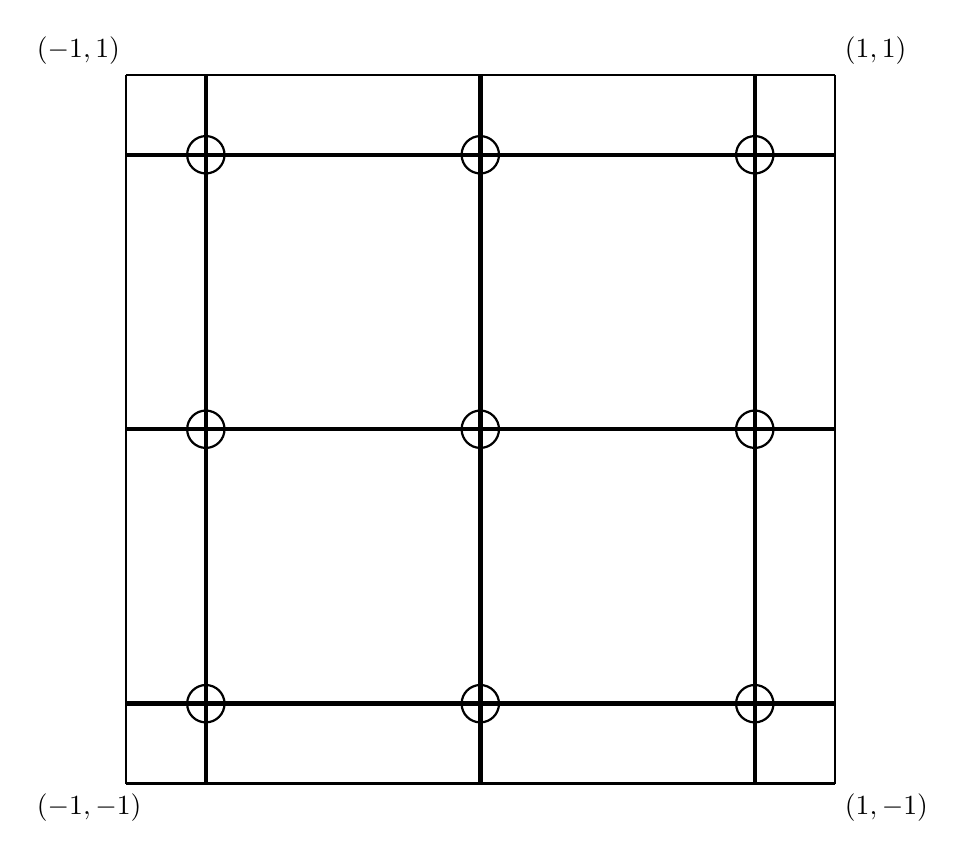
\begin{tikzpicture}[thick, scale=4.5]
	\draw[ultra thick] (-1,0) -- (1,0);
	\draw[ultra thick] (0,-1) -- (0,1);
	\draw[ultra thick] (-1,sqrt{0.6}) -- (1,sqrt{0.6});
	\draw[ultra thick] (sqrt{0.6},-1) -- (sqrt{0.6},1);
	\draw[ultra thick] (-1,-sqrt{0.6}) -- (1,-sqrt{0.6});
	\draw[ultra thick] (-sqrt{0.6},-1) -- (-sqrt{0.6},1);
	
	\draw[thick] (-1,-1) -- (1,-1);
	\draw[thick] (1,-1) -- (1,1);
	\draw[thick] (1,1) -- (-1,1);
	\draw[thick] (-1,1) -- (-1,-1);
	
	\draw (0,0) circle (1.5pt);
	\draw (-sqrt{0.6},0) circle (1.5pt);
	\draw (sqrt{0.6},0) circle (1.5pt);
	\draw (0,-sqrt{0.6}) circle (1.5pt);
	\draw (0,sqrt{0.6}) circle (1.5pt);
	\draw (-sqrt{0.6},-sqrt{0.6}) circle (1.5pt);
	\draw (sqrt{0.6},sqrt{0.6}) circle (1.5pt);
	\draw (sqrt{0.6},-sqrt{0.6}) circle (1.5pt);
	\draw (-sqrt{0.6},sqrt{0.6}) circle (1.5pt);
	
	
	\node[anchor=north east,text width=1cm] at (-1,-1) {$(-1,-1)$};
	\node[anchor=north west,text width=1cm] at (1,-1) {$(1,-1)$};
	\node[anchor=south east,text width=1cm] at (-1,1) {$(-1,1)$};
	\node[anchor=south west,text width=1cm] at (1,1) {$(1,1)$};
	\end{tikzpicture}
	\caption{Gaussian quadrature points $n=3$ for the standard quadrilateral element ${R_{st}} = {\left[ { - 1,1} \right]^2}$.}
\end{figure}
\newpage
\noindent
\textbf{Problem 4.2.} \textit{Let $n\ge m$ be two positive integers. Establish an error estimate for two-dimensional Gaussian quadrature defined by \eqref{4.6} which applies for a function $f \in {C^{2n}}\left( {\left[ { - 1,1} \right] \times \left[ { - 1,1} \right]} \right)$.}\\
\\
\textsc{Solution.} For each $y\in \left[-1,1\right]$, using $n$th Gaussian quadrature gives
\begin{align}
\label{4.9}
\int_{ - 1}^1 {f\left( {x,y} \right)dx}  = \sum\limits_{i = 1}^n {{w_{n,i}}f\left( {{x_{n,i}},y} \right)}  + \frac{2}{{\left( {2n + 1} \right)!}}{\left( {\frac{{{2^n}{{\left( {n!} \right)}^2}}}{{\left( {2n} \right)!}}} \right)^2}\frac{{{\partial ^{2n}}f}}{{\partial {x^{2n}}}}\left( {\xi \left( y \right),y} \right)
\end{align}
for some function
\begin{align}
\xi :\left[ { - 1,1} \right] &\to \left( { - 1,1} \right)\\
y &\mapsto \xi \left( y \right)
\end{align}
Integrating both sides of \eqref{4.9}, with respect to $y$, gives
\begin{align}
\int_{ - 1}^1 {\int_{ - 1}^1 {f\left( {x,y} \right)dx} dy}  =&\ \int_{ - 1}^1 {\left( {\sum\limits_{i = 1}^n {{w_{n,i}}f\left( {{x_{n,i}},y} \right)} } \right)dy} \\
 &+ \frac{2}{{\left( {2n + 1} \right)!}}{\left( {\frac{{{2^n}{{\left( {n!} \right)}^2}}}{{\left( {2n} \right)!}}} \right)^2}\int_{ - 1}^1 {\frac{{{\partial ^{2n}}f}}{{\partial {x^{2n}}}}\left( {\xi \left( y \right),y} \right)dy} \\
 =&\ \sum\limits_{i = 1}^n {{w_{n,i}}\int_{ - 1}^1 {f\left( {{x_{n,i}},y} \right)dy} }\label{4.14} \\
 &+ \frac{2}{{\left( {2n + 1} \right)!}}{\left( {\frac{{{2^n}{{\left( {n!} \right)}^2}}}{{\left( {2n} \right)!}}} \right)^2}\int_{ - 1}^1 {\frac{{{\partial ^{2n}}f}}{{\partial {x^{2n}}}}\left( {\xi \left( y \right),y} \right)dy} 
\end{align}
Use $m$th Gaussian quadrature for ${\int_{ - 1}^1 {f\left( {{x_{n,i}},y} \right)dy} }$ gives
\begin{align}
\label{4.16}
\int_{ - 1}^1 {f\left( {{x_{n,i}},y} \right)dy}  =&\ \sum\limits_{j = 1}^m {{w_{m,j}}f\left( {{x_{n,i}},{x_{m,j}}} \right)} \\
& + \frac{2}{{\left( {2m + 1} \right)!}}{\left( {\frac{{{2^m}{{\left( {m!} \right)}^2}}}{{\left( {2m} \right)!}}} \right)^2}\frac{{{\partial ^{2m}}f}}{{\partial {x^{2m}}}}\left( {{x_{n,i}},\eta \left( {{x_{n,i}}} \right)} \right)  \label{4.17}
\end{align}
for some function
\begin{align}
\eta :\left[ { - 1,1} \right] &\to \left( { - 1,1} \right)\\
x &\mapsto \eta \left( x \right)
\end{align}
Inserting \eqref{4.16}-\eqref{4.17} into \eqref{4.14} gives
\begin{align}
\label{4.20}
&\int_{ - 1}^1 {\int_{ - 1}^1 {f\left( {x,y} \right)dx} dy} \\
=&\ \sum\limits_{i = 1}^n {{w_{n,i}}\left( {\begin{array}{*{20}{l}}
{\sum\limits_{j = 1}^m {{w_{m,j}}f\left( {{x_{n,i}},{x_{m,j}}} \right)} }\\
{ + \dfrac{2}{{\left( {2m + 1} \right)!}}{{\left( {\dfrac{{{2^m}{{\left( {m!} \right)}^2}}}{{\left( {2m} \right)!}}} \right)}^2}\dfrac{{{\partial ^{2m}}f}}{{\partial {x^{2m}}}}\left( {{x_{n,i}},\eta \left( {{x_{n,i}}} \right)} \right)}
\end{array}} \right)} \\
& + \frac{2}{{\left( {2n + 1} \right)!}}{\left( {\frac{{{2^n}{{\left( {n!} \right)}^2}}}{{\left( {2n} \right)!}}} \right)^2}\int_{ - 1}^1 {\frac{{{\partial ^{2n}}f}}{{\partial {x^{2n}}}}\left( {\xi \left( y \right),y} \right)dy} \\
=&\ \sum\limits_{i = 1}^n {\sum\limits_{j = 1}^m {{w_{n,i}}{w_{m,j}}f\left( {{x_{n,i}},{x_{m,j}}} \right)} } \\
& + \frac{2}{{\left( {2m + 1} \right)!}}{\left( {\frac{{{2^m}{{\left( {m!} \right)}^2}}}{{\left( {2m} \right)!}}} \right)^2}\sum\limits_{i = 1}^n {{w_{n,i}}\frac{{{\partial ^{2m}}f}}{{\partial {x^{2m}}}}\left( {{x_{n,i}},\eta \left( {{x_{n,i}}} \right)} \right)} \\
& + \frac{2}{{\left( {2n + 1} \right)!}}{\left( {\frac{{{2^n}{{\left( {n!} \right)}^2}}}{{\left( {2n} \right)!}}} \right)^2}\int_{ - 1}^1 {\frac{{{\partial ^{2n}}f}}{{\partial {x^{2n}}}}\left( {\xi \left( y \right),y} \right)dy}   \label{4.25}
\end{align}
Define
\begin{align}
{E_{n,m}}\left\{ f \right\}: = \int_{ - 1}^1 {\int_{ - 1}^1 {f\left( {x,y} \right)dx} dy}  - \sum\limits_{i = 1}^n {\sum\limits_{j = 1}^m {{w_{n,i}}{w_{m,j}}f\left( {{x_{n,i}},{x_{m,j}}} \right)} } 
\end{align}
Then, we deduce from \eqref{4.20}-\eqref{4.25} that
\begin{align}
{E_{n,m}}\left\{ f \right\} =&\ \frac{2}{{\left( {2m + 1} \right)!}}{\left( {\frac{{{2^m}{{\left( {m!} \right)}^2}}}{{\left( {2m} \right)!}}} \right)^2}\sum\limits_{i = 1}^n {{w_{n,i}}\frac{{{\partial ^{2m}}f}}{{\partial {x^{2m}}}}\left( {{x_{n,i}},\eta \left( {{x_{n,i}}} \right)} \right)} \\
& + \frac{2}{{\left( {2n + 1} \right)!}}{\left( {\frac{{{2^n}{{\left( {n!} \right)}^2}}}{{\left( {2n} \right)!}}} \right)^2}\int_{ - 1}^1 {\frac{{{\partial ^{2n}}f}}{{\partial {x^{2n}}}}\left( {\xi \left( y \right),y} \right)dy} 
\end{align}

Since $f \in {C^{2n}}\left( {\left[ { - 1,1} \right] \times \left[ { - 1,1} \right]} \right)$ and $n\ge m$, we have the following estimate for ${E_{n,m}}\left\{ f \right\}$
\begin{align}
&\left| {{E_{n,m}}\left\{ f \right\}} \right|\\
& \le \frac{2}{{\left( {2m + 1} \right)!}}{\left( {\frac{{{2^m}{{\left( {m!} \right)}^2}}}{{\left( {2m} \right)!}}} \right)^2}\sum\limits_{i = 1}^n {{w_{n,i}}\left| {{{\frac{{{\partial ^{2m}}f}}{{\partial {x^{2m}}}}}}\left( {{x_{n,i}},\eta \left( {{x_{n,i}}} \right)} \right)} \right|} \\
& + \frac{2}{{\left( {2n + 1} \right)!}}{\left( {\frac{{{2^n}{{\left( {n!} \right)}^2}}}{{\left( {2n} \right)!}}} \right)^2}\int_{ - 1}^1 {\left| {{{\frac{{{\partial ^{2n}}f}}{{\partial {x^{2n}}}}}}\left( {\xi \left( y \right),y} \right)} \right|dy} \\
& \le \frac{2}{{\left( {2m + 1} \right)!}}{\left( {\frac{{{2^m}{{\left( {m!} \right)}^2}}}{{\left( {2m} \right)!}}} \right)^2}\sum\limits_{i = 1}^n {{w_{n,i}}} {\left\| {{{\frac{{{\partial ^{2m}}f}}{{\partial {x^{2m}}}}}}} \right\|_{{L^\infty }\left( {\left[ { - 1,1} \right]} \right)}}\\
& + \frac{2}{{\left( {2n + 1} \right)!}}{\left( {\frac{{{2^n}{{\left( {n!} \right)}^2}}}{{\left( {2n} \right)!}}} \right)^2}\int_{ - 1}^1 {{{\left\| {{{\frac{{{\partial ^{2n}}f}}{{\partial {x^{2n}}}}}}} \right\|}_{{L^\infty }\left( {\left[ { - 1,1} \right]} \right)}}dy} \\
=&\ \frac{1}{{\left( {2m + 1} \right)!}}{\left( {\frac{{{2^{m + 1}}{{\left( {m!} \right)}^2}}}{{\left( {2m} \right)!}}} \right)^2}{\left\| {{{\frac{{{\partial ^{2m}}f}}{{\partial {x^{2m}}}}}}} \right\|_{{L^\infty }\left( {\left[ { - 1,1} \right]} \right)}}\\
& + \frac{1}{{\left( {2n + 1} \right)!}}{\left( {\frac{{{2^{n + 1}}{{\left( {n!} \right)}^2}}}{{\left( {2n} \right)!}}} \right)^2}{\left\| {{{\frac{{{\partial ^{2n}}f}}{{\partial {x^{2n}}}}}}} \right\|_{{L^\infty }\left( {\left[ { - 1,1} \right]} \right)}}
\end{align} 

In particular, when $m=n$, we have the following two dimensional Gaussian quadrature for standard quadrilateral $R_{st}$.
\begin{align}
\int_{ - 1}^1 {\int_{ - 1}^1 {f\left( {x,y} \right)dx} dy}  = \sum\limits_{i = 1}^n {\sum\limits_{j = 1}^n {{w_{n,i}}{w_{n,j}}f\left( {{x_{n,i}},{x_{n,j}}} \right)} }  + {E_{n,n}}\left( f \right)
\end{align}
where
\begin{align}
{E_{n,n}}\left\{ f \right\} = \frac{2}{{\left( {2n + 1} \right)!}}{\left( {\frac{{{2^n}{{\left( {n!} \right)}^2}}}{{\left( {2n} \right)!}}} \right)^2}\left( \begin{array}{l}
\sum\limits_{i = 1}^n {{w_{n,i}}{{\dfrac{{{\partial ^{2n}}f}}{{\partial {x^{2n}}}}}}\left( {{x_{n,i}},\eta \left( {{x_{n,i}}} \right)} \right)} \\
 + \int_{ - 1}^1 {{{\dfrac{{{\partial ^{2n}}f}}{{\partial {x^{2n}}}}}}\left( {\xi \left( y \right),y} \right)dy} 
\end{array} \right)
\end{align}
satisfying the following estimate
\begin{align}
\left| {{E_{n,n}}\left\{ f \right\}} \right| \le \frac{2}{{\left( {2n + 1} \right)!}}{\left( {\frac{{{2^{n + 1}}{{\left( {n!} \right)}^2}}}{{\left( {2n} \right)!}}} \right)^2}{\left\| {{{\frac{{{\partial ^{2n}}f}}{{\partial {x^{2n}}}}}}} \right\|_{{L^\infty }\left( {\left[ { - 1,1} \right]} \right)}}
\end{align}
This finishes our derivation of error estimate for two-dimensional Gaussian quadrature for quadrilateral elements. \hfill $\square$
\subsection{Gaussian Quadrature for General Quadrilateral Elements}
Let $K$ be a quadrilateral element\index{quadrilateral element} with straight boundary lines and vertices $\left(x_i,y_i\right)$, $i=1,2,3,4$ arranged in the counter-clockwise order.
\begin{figure}[H]
	\centering
	\begin{tikzpicture}[thick, scale=4]
	\draw[thick,->] (-1.2,0) -- (1.2,0) node[anchor=north] {x};
	\draw[thick,->] (0,-1.2) -- (0,1.2) node[anchor=west] {y};
	
	\draw (-0.3,-1) -- (0.5,-0.5);
	\draw (0.5,-0.5) -- (0.7,0.9);
	\draw (0.7,0.9) -- (-0.8,0.2);
	\draw (-0.8,0.2) -- (-0.3,-1);
	
	\filldraw[black] (-0.3,-1) circle (0.5pt) node[anchor=east] {$P_1=(x_1,y_1)$};
	\filldraw[black] (0.5,-0.5) circle (0.5pt) node[anchor=west] {$P_2=(x_2,y_2)$};
	\filldraw[black] (0.7,0.9) circle (0.5pt) node[anchor=west] {$P_3=(x_3,y_3)$};
	\filldraw[black] (-0.8,0.2) circle (0.5pt) node[anchor=east] {$P_4=(x_4,y_4)$};
	
	\node[text width=0.5cm] at (0.4,0.4) {K};
	\end{tikzpicture}
\caption{A quadrilateral element with straight boundary lines.}
\end{figure}
We would like to evaluate
\begin{align}
I = \iint_K {f\left( {x,y} \right)dxdy}
\end{align}
The idea used here is very simple: First transform the quadrilateral element $K$ to the standard quadrilateral element $R_{st}$ and then apply the Gaussian quadrature \eqref{4.8}. To this end, we introduce the following nodal shape functions.\\
\\
\textbf{Definition 4.3.} Numbering four vertices $\left( { - 1, - 1} \right),\left( {1, - 1} \right),\left( {1,1} \right),\left( { - 1,1} \right)$ of ${R_{st}} = {\left[ { - 1,1} \right]^2}$ by (nodes) $1,2,3,4$, respectively. A collection of \textit{nodal shape functions for quadrilaterals}\index{nodal shape functions for quadrilaterals} is a collection of functions $N_i\left(\xi,\eta \right)$, $i=1,2,3,4$, satisfying
\begin{align}
\label{4.40}
{N_i}\left( {\xi ,\eta } \right) = \left\{ {\begin{array}{*{20}{l}}
{1,\mbox{ at node }i}\\
{0,\mbox{ at other nodes}}
\end{array}} \right., \hspace{0.2cm}i=1,2,3,4
\end{align}
\textbf{Problem 4.4.} \textit{Determine a collection of nodal shape function $N_i\left(\xi,\eta\right)$, $i=1,2,3,4$ for quadrilaterals explicitly.}\\
\\
\textsc{Solution.} There are a lot of choices of these nodal shape functions. We will find such a collection as easy as possible. First, we notice that there are four vertices at which functions $N_i$ attains their values. Reasonably, we will find $N_i$ as the following polynomials.
\begin{align}
\label{4.41}
{N_i}\left( {\xi ,\eta } \right) = {a_i}\xi \eta  + {b_i}\xi  + {c_i}\eta  + {d_i},\hspace{0.2cm} i = 1,2,3,4
\end{align}
Combing \eqref{4.40} with \eqref{4.41} gives a $4\times 4$ linear system of equations for four variables $a_i,b_i,c_i,d_i$, for each $i=1,2,3,4$. Solving these linear systems of equations for each $i=1,2,3,4$ gives
\begin{align}
\label{4.42}
{N_1}\left( {\xi ,\eta } \right) =&\ \frac{1}{4}\left( {1 - \xi } \right)\left( {1 - \eta } \right)\\
{N_2}\left( {\xi ,\eta } \right) =&\ \frac{1}{4}\left( {1 + \xi } \right)\left( {1 - \eta } \right)\\
{N_3}\left( {\xi ,\eta } \right) =&\ \frac{1}{4}\left( {1 + \xi } \right)\left( {1 + \eta } \right)\\
{N_4}\left( {\xi ,\eta } \right) =&\ \frac{1}{4}\left( {1 - \xi } \right)\left( {1 + \eta } \right) \label{4.45}
\end{align}
Therefore, we obtain a collection of nodal shape functions for quadrilaterals given by \eqref{4.42}-\eqref{4.45}. \hfill $\square$\\

We now construct a \textit{bilinear mapping} to map the quadrilateral element $K$ with straight boundary lines to the standard quadrilateral element $R_{st}$. Such a mapping can be achieved conveniently by using the nodal shape functions \eqref{4.42}-\eqref{4.45} as follows.

Consider the following bilinear mapping $S$.
\begin{align}
S:{\mathbb{R}^2} &\to {\mathbb{R}^2}\\
\left( {\xi ,\eta } \right) &\mapsto \left( {x,y} \right) := S\left( {\xi ,\eta } \right) = \left( {{S_1}\left( {\xi ,\eta } \right),{S_2}\left( {\xi ,\eta } \right)} \right)
\end{align}
where $S_1,S_2$ are defined by
\begin{align}
{S_1}\left( {\xi ,\eta } \right) =&\ \sum\limits_{i = 1}^4 {{x_i}{N_i}\left( {\xi ,\eta } \right)} \\
 =&\ \frac{1}{4}\sum\limits_{i = 1}^4 {{x_i}}  + \frac{{ - {x_1} + {x_2} + {x_3} - {x_4}}}{4}\xi \\
& + \frac{{ - {x_1} - {x_2} + {x_3} + {x_4}}}{4}\eta  + \frac{{{x_1} - {x_2} + {x_3} - {x_4}}}{4}\xi \eta \\
{S_2}\left( {\xi ,\eta } \right)=&\ \sum\limits_{i = 1}^4 {{x_i}{N_i}\left( {\xi ,\eta } \right)} \\
=&\ \frac{1}{4}\sum\limits_{i = 1}^4 {{y_i}}  + \frac{{ - {y_1} + {y_2} + {y_3} - {y_4}}}{4}\xi \\
& + \frac{{ - {y_1} - {y_2} + {y_3} + {y_4}}}{4}\eta  + \frac{{{y_1} - {y_2} + {y_3} - {y_4}}}{4}\xi \eta 
\end{align}
\begin{figure}[H]
	\centering
	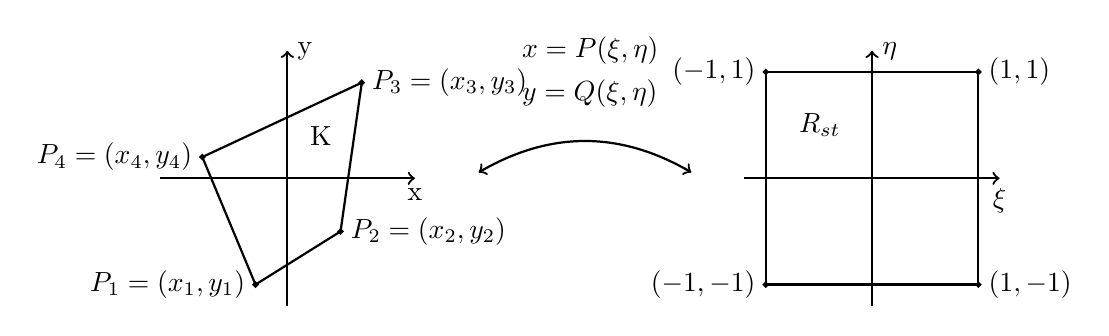
\begin{tikzpicture}[thick, scale=1.35]
		\begin{scope}
			\draw[thick,->] (-1.2,0) -- (1.2,0) node[anchor=north] {x};
			\draw[thick,->] (0,-1.2) -- (0,1.2) node[anchor=west] {y};
			
			\draw (-0.3,-1) -- (0.5,-0.5);
			\draw (0.5,-0.5) -- (0.7,0.9);
			\draw (0.7,0.9) -- (-0.8,0.2);
			\draw (-0.8,0.2) -- (-0.3,-1);
			
			\filldraw[black] (-0.3,-1) circle (0.5pt) node[anchor=east] {$P_1=(x_1,y_1)$};
			\filldraw[black] (0.5,-0.5) circle (0.5pt) node[anchor=west] {$P_2=(x_2,y_2)$};
			\filldraw[black] (0.7,0.9) circle (0.5pt) node[anchor=west] {$P_3=(x_3,y_3)$};
			\filldraw[black] (-0.8,0.2) circle (0.5pt) node[anchor=east] {$P_4=(x_4,y_4)$};
	
			\node[text width=0.5cm] at (0.4,0.4) {K};
		\end{scope}
	
		\begin{scope}[xshift=2.8cm]
			\node[anchor=east] at (-1,0) (A) {};
			\node[anchor=west] at (1,0) (B) {};
			\draw (B) edge[bend right=30,<->] (A);
			\node[text width=2cm] at (0.15,0.8) {$y=Q(\xi,\eta)$};
			\node[text width=2cm] at (0.15,1.2) {$x=P(\xi,\eta)$};
		\end{scope}
	
		\begin{scope}[xshift=5.5cm]
			\draw[thick,->] (-1.2,0) -- (1.2,0) node[anchor=north] {$\xi$};
			\draw[thick,->] (0,-1.2) -- (0,1.2) node[anchor=west] {$\eta$};
			
			\draw (-1,-1) -- (1,-1);
			\draw (1,-1) -- (1,1);
			\draw (1,1) -- (-1,1);
			\draw (-1,1) -- (-1,-1);
			
			\filldraw[black] (-1,-1) circle (0.5pt) node[anchor=east] {$(-1,-1)$};
			\filldraw[black] (1,-1) circle (0.5pt) node[anchor=west] {$(1,-1)$};
			\filldraw[black] (1,1) circle (0.5pt) node[anchor=west] {$(1,1)$};
			\filldraw[black] (-1,1) circle (0.5pt) node[anchor=east] {$(-1,1)$};
			
			\node[text width=0.5cm] at (-0.5,0.5) {$R_{st}$};
		\end{scope}
	\end{tikzpicture}
	\caption{Bilinear mapping between $K$ and $R_{st}$.}
\end{figure}

It is easy to verify that $S$ transforms the standard quadrilateral $R_{st}$ into the quadrilateral element $K$, i.e.,
\begin{align}
S:{R_{st}} \mapsto K
\end{align}
Thus, we have
\begin{align}
\iint_K {f\left( {x,y} \right)dxdy} = \iint_{{R_{st}}} {f\left( {S_1\left( {\xi ,\eta } \right),S_2\left( {\xi ,\eta } \right)} \right)\left| {J\left( {\xi ,\eta } \right)} \right|d\xi d\eta }
\end{align}
where ${J\left( {\xi ,\eta } \right)}$ is the Jacobian\index{Jacobian} of the transformation defined by
\begin{align}
J\left( {\xi ,\eta } \right) =&\ \frac{{\partial \left( {x,y} \right)}}{{\partial \left( {\xi ,\eta } \right)}}\\
 =&\ \det \left[ {\begin{array}{*{20}{c}}
{\dfrac{{\partial x}}{{\partial \xi }}}&{\dfrac{{\partial x}}{{\partial \eta }}}\\
{\dfrac{{\partial y}}{{\partial \xi }}}&{\dfrac{{\partial y}}{{\partial \eta }}}
\end{array}} \right]
\end{align}
We compute this Jacobian explicitly as follows.
\begin{align}
\left| {J\left( {\xi ,\eta } \right)} \right| =&\ \left| {\dfrac{{\partial {S_1}}}{{\partial \xi }}\left( {\xi ,\eta } \right)\dfrac{{\partial {S_2}}}{{\partial \eta }}\left( {\xi ,\eta } \right) - \dfrac{{\partial {S_1}}}{{\partial \eta }}\left( {\xi ,\eta } \right)\dfrac{{\partial {S_2}}}{{\partial \xi }}\left( {\xi ,\eta } \right)} \right|\\
=&\ \left| \begin{array}{l}
\left( {\dfrac{{ - {x_1} + {x_2} + {x_3} - {x_4}}}{4} + \dfrac{{{x_1} - {x_2} + {x_3} - {x_4}}}{4}\eta } \right) \cdot \\
 \cdot \left( {\dfrac{{ - {y_1} - {y_2} + {y_3} + {y_4}}}{4} + \dfrac{{{y_1} - {y_2} + {y_3} - {y_4}}}{4}\xi } \right)\\
 - \left( {\dfrac{{ - {x_1} - {x_2} + {x_3} + {x_4}}}{4} + \dfrac{{{x_1} - {x_2} + {x_3} - {x_4}}}{4}\xi } \right) \cdot \\
 \cdot \left( {\dfrac{{ - {y_1} + {y_2} + {y_3} - {y_4}}}{4} + \dfrac{{{y_1} - {y_2} + {y_3} - {y_4}}}{4}\eta } \right)
\end{array} \right|\\
=&\ \left| \begin{array}{l}
\dfrac{{{x_1}{y_2} - {x_2}{y_1} + {x_2}{y_3} - {x_3}{y_2} + {x_3}{y_4} - {x_4}{y_3} + {x_4}{y_1} - {x_1}{y_4}}}{8}\\
 + \dfrac{{{x_1}{y_4} - {x_4}{y_1} + {x_2}{y_3} - {x_3}{y_2} + {x_3}{y_1} - {x_1}{y_3} + {x_4}{y_2} - {x_2}{y_4}}}{8}\xi \\
 + \dfrac{{{x_1}{y_3} - {x_3}{y_1} + {x_2}{y_1} - {x_1}{y_2} + {x_3}{y_4} - {x_4}{y_3} + {x_4}{y_2} - {x_2}{y_4}}}{8}\eta 
\end{array} \right|
\end{align}

Applying the Gaussian quadrature \eqref{4.8} for the standard quadrilateral element yields the following formula.\\
\\
\textsc{Gaussian Quadrature of Order $n$ for General Quadrilateral Elements $K$.}
\begin{align}
\iint_K {f\left( {x,y} \right)dxdy} \approx \sum\limits_{i = 1}^n {\sum\limits_{j = 1}^n {{w_{n,i}}{w_{n,j}}f\left( {S_1\left( {{x_{n,i}},{x_{n,j}}} \right),S_2\left( {{x_{n,i}},{x_{n,j}}} \right)} \right)\left| {J\left( {{x_{n,i}},{x_{n,j}}} \right)} \right|} } 
\end{align}

\section{Two-Dimensional Gaussian Quadrature for Triangular Elements}
\subsection{Gaussian Quadrature for the Standard Triangular Element ${T_{st}}$}
From now on, we will call $T_{st}= \left\{ {\left( {\xi ,\eta } \right):0 \le \xi ,\eta ,\xi  + \eta  \le 1} \right\}$ the standard triangular element.
\begin{figure}[H]
	\centering
	\begin{tikzpicture}[scale=4]
	\draw[thin,->] (-0.2,0) -- (1.2,0) node[anchor=north] {$\xi$};
	\draw[thin,->] (0,-0.2) -- (0,1.2) node[anchor=west] {$\eta$};
	
	\draw[thick] (0,0) -- (0,1);
	\draw[thick] (0,0) -- (1,0);
	\draw[thick] (1,0) -- (0,1);
	
%	\filldraw[black] (0,0) circle (0.5pt) node[anchor=north west] {$(0,0)$};
%	\filldraw[black] (0,1) circle (0.5pt) node[anchor=east] {$(0,1)$};
%	\filldraw[black] (1,0) circle (0.5pt) node[anchor=north] {$(1,0)$};
	
	\node[anchor=north west,text width=0.8cm] at (0,0) {$(0,0)$};
	\node[anchor=east,text width=0.8cm] at (0,1) {$(0,1)$};
	\node[anchor=north,text width=0.8cm] at (1,0) {$(1,0)$};
	
	\node[text width=0.5cm] at (0.3,0.3) {$T_{st}$};
	\end{tikzpicture}
\caption{The standard triangular element $T_{st}$.}
\end{figure}
We need to approximate
\begin{align}
I =&\ \iint_{{T_{st}}} {f\left( {\xi ,\eta } \right)d\xi d\eta }  \cr 
  =&\ \int_0^1 {\int_0^{1 - \eta } f \left( {\xi ,\eta } \right)d\xi d\eta }   \cr 
  =&\ \int_0^1 {\int_0^{1 - \xi } f \left( {\xi ,\eta } \right)d\eta d\xi } 
\end{align}
\subsubsection{Tensor Product-Type Gaussian Quadrature.}
The idea is that we will transform the standard triangular element\index{standard triangular element} $T_{st}$ to the standard quadrilateral element\index{standard quadrilateral element} $R_{st}$, and then apply the Gaussian quadrature for $R_{st}$. 

We consider such a transformation
\begin{align}
\widetilde S:{R_{st}}\backslash \left( {\left[ { - 1,1} \right] \times \left\{ 1 \right\}} \right) &\to {T_{st}}\backslash \left\{ {\left( {1,1} \right)} \right\}\\
\left( {x,y} \right) &\mapsto \left( {\xi ,\eta } \right): = \widetilde S\left( {x,y} \right) = \left( {{{\widetilde S}_1}\left( {x,y} \right),{{\widetilde S}_2}\left( {x,y} \right)} \right)
\end{align}
where $\widetilde{S}_1,\widetilde{S}_2$ are defined by
\begin{align}
{\widetilde S_1}\left( {x,y} \right) =&\ \frac{{\left( {1 + x} \right)\left( {1 - y} \right)}}{4}\\
{\widetilde S_2}\left( {x,y} \right) =&\ \frac{{1 + y}}{2}
\end{align}

It is easy to verify that this bilinear mapping $\widetilde S$ is a bijection from\\
${R_{st}}\backslash \left( {\left[ { - 1,1} \right] \times \left\{ 1 \right\}} \right)$ into ${T_{st}}\backslash \left\{ {\left( {1,1} \right)} \right\}$. The inverse mapping of $\widetilde S$ is given by
\begin{align}
{\widetilde S^{ - 1}}:{T_{st}}\backslash \left\{ {\left( {1,1} \right)} \right\} &\to {R_{st}}\backslash \left( {\left[ { - 1,1} \right] \times \left\{ 1 \right\}} \right)\\
\left( {\xi ,\eta } \right) &\mapsto \left( {x,y} \right): = {\widetilde S^{ - 1}}\left( {\xi ,\eta } \right) = \left( {\widetilde S_1^{ - 1}\left( {\xi ,\eta } \right),\widetilde S_2^{ - 1}\left( {\xi ,\eta } \right)} \right)
\end{align}
where
\begin{align}
\widetilde S_1^{ - 1}\left( {\xi ,\eta } \right) =&\ \frac{{2\xi }}{{1 - \eta }} - 1\\
\widetilde S_2^{ - 1}\left( {\xi ,\eta } \right) =&\ 2\eta  - 1
\end{align}
\begin{figure}[H]
	\centering
	\begin{tikzpicture}[scale=1.3]
	\begin{scope}
	\draw[thin,->] (-1.2,0) -- (1.2,0) node[anchor=south west] {$a$};
	\draw[thin,->] (0,-1.2) -- (0,1.2) node[anchor=south] {$b$};
	
	\draw[thick] (-1,-1) -- (1,-1);
	\draw[thick] (1,-1) -- (1,1);
	\draw[thick] (1,1) -- (-1,1);
	\draw[thick] (-1,1) -- (-1,-1);
	
	\node[anchor=south west,text width=0.8cm] at (0,1) {$1$};
	\node[anchor=north west,text width=0.8cm] at (1,0) {$1$};
	\node[anchor=north east,text width=0.3cm] at (-1,0) {$-1$};
	\node[anchor=north west,text width=0.8cm] at (0,-1) {$-1$};
	\end{scope}
	
	\begin{scope}[xshift=3cm]
	\node[anchor=east] at (-2.7,0.3) (A) {};
	\node[anchor=west] at (3.3,0.3) (B) {};
	\draw (B) edge[bend right=15,<-] (A);
	\end{scope}
	
	\begin{scope}[xshift=6cm,yshift=-1cm,scale=2]
	\draw[thin,->] (-0.2,0) -- (1.2,0) node[anchor=north] {$\xi$};
	\draw[thin,->] (0,-0.2) -- (0,1.2) node[anchor=west] {$\eta$};
	
	\draw[thick] (0,0) -- (0,1);
	\draw[thick] (0,0) -- (1,0);
	\draw[thick] (1,0) -- (0,1);
	
	\node[anchor=north west,text width=0.8cm] at (0,0) {$B$};
	\node[anchor=west,text width=0.8cm] at (0,1) {$C$};
	\node[anchor=east,text width=0.3cm] at (0,1) {$1$};
	\node[anchor=south west,text width=0.8cm] at (1,0) {$A$};
	\node[anchor=north west,text width=0.8cm] at (1,0) {$1$};
	
	\node[text width=0.5cm] at (0.3,0.3) {$T_{0}$};
	\end{scope}
	\end{tikzpicture}
\caption{Illustration of the mapping between the square $R_{st}$ and the triangle $T_{st}$.}
\end{figure}

The transformation $\widetilde S$ basically ``collapses'' the top edge of the square $R_{st}$ into the top vertex $\left(0,1\right)$ of the triangle $T_{st}$. The Jacobians of the transformations are
\begin{align}
\widetilde J\left( {x,y} \right) =&\ \frac{{\partial \left( {\xi ,\eta } \right)}}{{\partial \left( {x,y} \right)}}\\
 =&\ \det \left[ {\begin{array}{*{20}{c}}
{\dfrac{{\partial \xi }}{{\partial x}}}&{\dfrac{{\partial \xi }}{{\partial y}}}\\
{\dfrac{{\partial \eta }}{{\partial x}}}&{\dfrac{{\partial \eta }}{{\partial y}}}
\end{array}} \right]
\end{align}
Thus,
\begin{align}
\left| {\widetilde J\left( {x,y} \right)} \right| =&\ \left| {\frac{{\partial {{\widetilde S}_1}}}{{\partial x}}\left( {x,y} \right)\frac{{\partial {{\widetilde S}_2}}}{{\partial y}}\left( {x,y} \right) - \frac{{\partial {{\widetilde S}_1}}}{{\partial y}}\left( {x,y} \right)\frac{{\partial {{\widetilde S}_2}}}{{\partial x}}\left( {x,y} \right)} \right|\\
 =&\ \left| {\frac{{1 - y}}{4} \cdot \frac{1}{2} + \frac{{1 + x}}{4} \cdot 0} \right|\\
 =&\ \frac{{1 - y}}{8}
\end{align}
and
\begin{align}
{\widetilde J^{ - 1}}\left( {\xi ,\eta } \right) =&\ \frac{{\partial \left( {x,y} \right)}}{{\partial \left( {\xi ,\eta } \right)}}\\
 =&\ \det \left[ {\begin{array}{*{20}{c}}
{\dfrac{{\partial x}}{{\partial \xi }}}&{\dfrac{{\partial x}}{{\partial \eta }}}\\
{\dfrac{{\partial y}}{{\partial \xi }}}&{\dfrac{{\partial y}}{{\partial \eta }}}
\end{array}} \right]
\end{align}
Thus,
\begin{align}
\left| {{{\widetilde J}^{ - 1}}\left( {\xi ,\eta } \right)} \right| =&\ \left| {\frac{{\partial \widetilde S_1^{ - 1}}}{{\partial \xi }}\left( {\xi ,\eta } \right) \cdot \frac{{\partial \widetilde S_2^{ - 1}}}{{\partial \eta }}\left( {\xi ,\eta } \right) - \frac{{\partial \widetilde S_1^{ - 1}}}{{\partial \eta }}\left( {\xi ,\eta } \right) \cdot \frac{{\partial \widetilde S_2^{ - 1}}}{{\partial \xi }}\left( {\xi ,\eta } \right)} \right|\\
=&\ \left| {\frac{2}{{1 - \eta }} \cdot 2 - 0 \cdot \frac{{2\xi }}{{{{\left( {1 - \eta } \right)}^2}}}} \right|\\
 =&\ \frac{4}{{1 - \eta }}
\end{align}
\textbf{Remark 5.1.} The quantity $\left| {{{\widetilde J}^{ - 1}}\left( {\xi ,\eta } \right)} \right|$ can be computed shorter as follows.
\begin{align}
\left| {{{\widetilde J}^{ - 1}}\left( {\xi ,\eta } \right)} \right| =&\ \frac{1}{{\left| {\widetilde J\left( {x,y} \right)} \right|}}\\
=&\ \frac{8}{{1 - y}}\\
=&\ \frac{4}{{1 - \eta }}
\end{align}

Return to our problem, under the transformation $\widetilde S$, we have
\begin{align}
  \iint_{{T_{st}}} {f\left( {\xi ,\eta } \right)d\xi d\eta } =&\ \iint_{{R_{st}}} {f\left( {{{\widetilde S}_1}\left( {x,y} \right),{{\widetilde S}_2}\left( {x,y} \right)} \right)\left| {\widetilde J\left( {x,y} \right)} \right|dxdy}\\
   =&\ \iint_{{R_{st}}} {f\left( {\frac{{\left( {1 + x} \right)\left( {1 - y} \right)}}{4},\frac{{1 + y}}{2}} \right)\frac{{1 - y}}{8}dxdy} \label{5.24}
\end{align}
Applying \eqref{4.8} to the integral \eqref{5.24} yields the following results.\\
\\
\textsc{Gaussian Quadrature of order $n$ for Standard triangular element $T_{st}$.}
\begin{align}
\iint_{{T_{st}}} {f\left( {\xi ,\eta } \right)d\xi d\eta } \approx \sum\limits_{i = 1}^n {\sum\limits_{j = 1}^n {{w_{n,i}}{w_{n,j}}\frac{{1 - {x_{n,j}}}}{8}f\left( {\frac{{\left( {1 + {x_{n,i}}} \right)\left( {1 - {x_{n,j}}} \right)}}{4},\frac{{1 + {x_{n,j}}}}{2}} \right)} } 
\end{align}

Conversely, we also obtain the following result.
\begin{align}
\label{5.26}
  \iint_{{R_{st}}} {f\left( {x,y} \right)dxdy} =&\ \iint_{{T_{st}}} {f\left( {\widetilde S_1^{ - 1}\left( {\xi ,\eta } \right),\widetilde S_2^{ - 1}\left( {\xi ,\eta } \right)} \right)\left| {{{\widetilde J}^{ - 1}}\left( {\xi ,\eta } \right)} \right|d\xi d\eta } \\
  =&\ \iint_{{T_{st}}} {\frac{4}{{1 - \eta }}f\left( {\frac{{2\xi }}{{1 - \eta }} - 1,2\eta  - 1} \right)d\xi d\eta } \label{5.27}
\end{align}
\textbf{Remark 5.2.} The transformation $\widetilde S$ is bilinear and the corresponding Jacobian ${\widetilde J\left( {x,y} \right)}$ is bounded, for instance, 
\begin{align}
\left| {\widetilde J\left( {x,y} \right)} \right| = \frac{{1 - y}}{8} \le \frac{1}{4},\hspace{0.2cm}\forall \left( {x,y} \right) \in {R_{st}}\backslash \left( {\left[ { - 1,1} \right] \times \left\{ 1 \right\}} \right)
\end{align}
However, its inverse mapping, $\widetilde{S}^{-1}$, is non-linear, and its Jacobian has a singularity at $\left(\xi,\eta \right)=\left(0,1\right)$. Hence, this Jacobian ${{{\widetilde J}^{ - 1}}\left( {\xi ,\eta } \right)}$ and \eqref{5.26}-\eqref{5.27} are not used.\\
\\
\textbf{Remark 5.3.} \textit{``Tensor product-type quadrature\index{tensor product-type quadrature} have several advantages. In particular, their derivation and application is straightforward. They are versatile in that many one-dimensional rules are available for several different integrands. Extremely high-order polynomials may be evaluated, although precision may be limited since most references provide points and weights to 20 significant digits at most. The primary disadvantage is inefficiency since for high $N$, a relatively large number of points is required, and other quadrature rules are available with many fewer points. The secondary disadvantage is that the location of the points is unsymmetrical. Except for rules of low order, a large number of points will be concentrated in a relatively small region near one vertex (the top $\left(0,1\right)$ vertex). Such an arrangement, although correct, maybe considered aesthetically undesirable.''}\footnote{Quoted in \cite{7}.}
\subsubsection{Symmetrical Gaussian Quadrature on Triangles}
The goal is to develop quadrature rules of the form
\begin{align}
\label{5.29}
\iint_{{T_{st}}} {f\left( {\xi ,\eta } \right)d\xi d\eta } \approx \frac{1}{2}\sum\limits_{i = 1}^{{N_T}} {{w_{{N_T},i}}f\left( {{\xi _{{N_T},i}},{\eta _{{N_T},i}}} \right)}
\end{align}
where $N_T$ is the number of quadrature points\index{quadrature points},${\left( {{\xi _{{N_T},i}},{\eta _{{N_T},i}}} \right)}$ are quadrature points located inside the standard triangle\index{standard triangle} and $w_{{N_T},i}$ are weights (normalized with respect to the triangle area). In addition to the criteria that the resulting quadrature should use as less as possible number of quadrature points to achieve as high as possible accuracy, we also would like the quadrature points possess some kind of symmetry.

The basic idea is the same as that used in developing Gaussian quadrature for the standard interval $\left[-1,1\right]$. We want to choose points $\left( {{\xi _{{N_T},i}},{\eta _{{N_T},i}}} \right)$ and weights $w_{{N_T},i}$ in \eqref{5.29} so that the quadrature \eqref{5.29} is as accurate as possible in some sense. Generally speaking, a \textit{Gaussian quadrature of degree $n$ for triangles} is defined as a quadrature of \eqref{5.29} that is exact for arbitrary polynomial of degree $n$, namely,
\begin{align}
\iint_{{T_{st}}} {f\left( {\xi ,\eta } \right)d\xi d\eta } \approx \frac{1}{2}\sum\limits_{i = 1}^{{N_T}} {{w_{{N_T},i}}f\left( {{\xi _{{N_T},i}},{\eta _{{N_T},i}}} \right)} ,\hspace{0.2cm}\forall g\left( {\xi ,\eta } \right) \in {\mathbb{P}_n}\left( {\xi ,\eta } \right)
\end{align}
where ${\mathbb{P}_n}\left( {\xi ,\eta } \right)$ represents the complete polynomial space of degree $n$ in two dimensions
\begin{align}
{\mathbb{P}_n}\left( {\xi ,\eta } \right) = \mbox{span}\left\{ {{\xi ^i}{\eta ^j}:0 \leqslant i,j,i + j \leqslant n} \right\}
\end{align}
For example,
\begin{align}
{\mathbb{P}_1}\left( {\xi ,\eta } \right) =&\ \mbox{span}\left\{ {1,\xi ,\eta } \right\}\\
{\mathbb{P}_2}\left( {\xi ,\eta } \right) =&\ \mbox{span}\left\{ {1,\xi ,\eta ,{\xi ^2},\xi \eta ,{\eta ^2}} \right\}
\end{align}
Note that 
\begin{align}
\dim \left( {{\mathbb{P}_n}} \right) = \frac{{\left( {n + 1} \right)\left( {n + 2} \right)}}{2}
\end{align}
Indeed, for each $i=0,1,\ldots,n$, $j$ can only equal to $0,1,\ldots,n-i$. That means, there are exactly $n+1-i$ choices of $j$ for each $i=0,1,\ldots,n$, $j$. Thus,
\begin{align}
\dim \left( {{\mathbb{P}_n}} \right)=&\ \sum\limits_{i = 0}^n {\left( {n + 1 - i} \right)} \\
 =&\ \sum\limits_{i = 1}^{n + 1} i \\
=&\ \frac{{\left( {n + 1} \right)\left( {n + 2} \right)}}{2}
\end{align}
\textbf{Problem 5.4.} \textit{Prove that}
\begin{align}
\label{5.38}
\iint_{{T_{st}}} {{\xi ^i}{\eta ^j}d\xi d\eta } = \frac{{i!j!}}{{\left( {i + j + 2} \right)!}},\hspace{0.2cm}0 \le i,j,i + j \le n
\end{align}
\textsc{Proof.} Integration by parts formula is the main tool we use here.
\begin{align}
\iint_{{T_{st}}} {{\xi ^i}{\eta ^j}d\xi d\eta } =&\ \int_0^1 {\int_0^{1 - \eta } {{\xi ^i}{\eta ^j}d\xi d\eta } } \\
 =&\ \int_0^1 {{\eta ^j}\frac{{{{\left( {1 - \eta } \right)}^{i + 1}}}}{{i + 1}}d\eta } \\
 =&\ \int_0^1 {\frac{{{\eta ^{j + 1}}}}{{j + 1}}{{\left( {1 - \eta } \right)}^i}d\eta } \\
 =&\ \int_0^1 {\frac{{{\eta ^{j + 2}}}}{{\left( {j + 1} \right)\left( {j + 2} \right)}}i{{\left( {1 - \eta } \right)}^{i - 1}}d\eta } \\
 =&\  \cdots \\
 =&\ \int_0^1 {\frac{{{\eta ^{j + 1}}}}{{\prod\limits_{k = j + 1}^{i + j + 1} k }}i!d\eta } \\
 =&\ \frac{{i!j!}}{{\left( {i + j + 1} \right)!}}\int_0^1 {{\eta ^{j + 1}}d\eta } \\
 =&\ \frac{{i!j!}}{{\left( {i + j + 2} \right)!}}
\end{align}
for all $0 \le i,j,i + j \le n$.\hfill $\square$\\
\\
\textbf{5.1.2.1. Gaussian Quadrature of Degree 1 for Triangles.}\\
\\
By definition, the quadrature should be accurate for $f\left( {\xi ,\eta } \right) = 1,\xi$ and $\eta $. Plugging these into \eqref{5.29}, with the help of \eqref{5.38}, yields the following system of equations.
\begin{align}
\label{5.47}
\sum\limits_{i = 1}^{{N_T}} {{w_{{N_T},i}}}  =&\ 1\\
\sum\limits_{i = 1}^{{N_T}} {{w_{{N_T},i}}{\xi _{{N_T},i}}}  =&\ \frac{1}{3}\\
\sum\limits_{i = 1}^{{N_T}} {{w_{{N_T},i}}{\eta _{{N_T},i}}}  =&\ \frac{1}{3} \label{5.49}
\end{align}

It must be emphasized here that \eqref{5.47}-\eqref{5.49} has infinitely many solutions. But for efficiency, we will choose $N_T$ as the smallest positive integer such that \eqref{5.47}-\eqref{5.49} has at least one solution.\\
\\
\textsc{Solve \eqref{5.47}-\eqref{5.49} when choosing $N_T=1$.} 

For $N_T=1$, \eqref{5.47}-\eqref{5.49} becomes
\begin{align}
{w_{1,1}} =&\ 1\\
{w_{1,1}}{\xi _{1,1}} =&\ \frac{1}{3}\\
{w_{1,1}}{\eta _{1,1}} =&\ \frac{1}{3}
\end{align}
Thus, 
\begin{align}
{N_T} =&\ 1\\
{w_{1,1}} =&\ 1\\
{\xi _{1,1}} =&\ \frac{1}{3}\\
{\eta _{1,1}} =&\ \frac{1}{3}
\end{align}
is a solution of \eqref{5.47}-\eqref{5.49}. Therefore, we obtain the following formula.\\
\\
\textsc{Gaussian Quadrature of Degree 1 for the Standard Triangle $T_{st}$.}
\begin{align}
\iint_{{T_{st}}} {f\left( {\xi ,\eta } \right)d\xi d\eta } \approx \frac{1}{2}f\left( {\frac{1}{3},\frac{1}{3}} \right)
\end{align}
\textbf{5.1.2.2. Gaussian Quadrature of Degree 2 for Triangles.}\\
\\
Plugging $f\left( {\xi ,\eta } \right) = 1,\xi ,\eta ,{\xi ^2},\xi \eta$ and ${\eta ^2}$ into \eqref{5.29}, with the help of \eqref{5.38}, yields the following system of equations.
\begin{align}
\label{5.58}
\sum\limits_{i = 1}^{{N_T}} {{w_{{N_T},i}}}  =&\ 1\\
\sum\limits_{i = 1}^{{N_T}} {{w_{{N_T},i}}{\xi _{{N_T},i}}}  =&\ \frac{1}{3}\\
\sum\limits_{i = 1}^{{N_T}} {{w_{{N_T},i}}{\eta _{{N_T},i}}}  =&\ \frac{1}{3}\\
\sum\limits_{i = 1}^{{N_T}} {{w_{{N_T},i}}\xi _{{N_T},i}^2}  =&\ \frac{1}{6}\\
\sum\limits_{i = 1}^{{N_T}} {{w_{{N_T},i}}\eta _{{N_T},i}^2}  =&\ \frac{1}{6}\\
\sum\limits_{i = 1}^{{N_T}} {{w_{{N_T},i}}{\xi _{{N_T},i}}{\eta _{{N_T},i}}}  =&\ \frac{1}{{12}} \label{5.63}
\end{align}
It is obvious that $N_T=1$ will not work, i.e., \eqref{5.58}-\eqref{5.63} has no solution (try it!).\\
\\
\textsc{Solve \eqref{5.58}-\eqref{5.63} when choosing $N_T=2$.}

For $N_T=2$, \eqref{5.58}-\eqref{5.63} becomes
\begin{align}
\label{5.64}
{w_{2,1}} + {w_{2,2}} =&\ 1\\
{w_{2,1}}{\xi _{2,1}} + {w_{2,2}}{\xi _{2,2}} =&\ \frac{1}{3}\label{5.65}\\
{w_{2,1}}{\eta _{2,1}} + {w_{2,2}}{\eta _{2,2}} =&\ \frac{1}{3}\label{5.66}\\
{w_{2,1}}\xi _{2,1}^2 + {w_{2,2}}\xi _{2,2}^2 =&\ \frac{1}{6}\label{5.67}\\
{w_{2,1}}\eta _{2,1}^2 + {w_{2,2}}\eta _{2,2}^2 =&\ \frac{1}{6}\label{5.68}\\
{w_{2,1}}{\xi _{2,1}}{\eta _{2,1}} + {w_{2,2}}{\xi _{2,2}}{\eta _{2,2}} =&\ \frac{1}{{12}} \label{5.69}
\end{align}
It is obvious that ${\xi _{2,1}} \ne {\xi _{2,2}}$. Indeed, suppose for the contrary that ${\xi _{2,1}} = {\xi _{2,2}}$, \eqref{5.64}-\eqref{5.65} implies ${\xi _{2,1}} = {\xi _{2,2}} = \frac{1}{3}$, but this contradicts to \eqref{5.67}. Thus, ${\xi _{2,1}} \ne {\xi _{2,2}}$. Similarly, we have ${\eta _{2,1}} \ne {\eta _{2,2}}$.

Solving for $w_{2,1},w_{2,2}$ in terms of $\xi _{2,1},\xi _{2,2}$ via \eqref{5.64}-\eqref{5.65} gives
\begin{align}
\label{5.70}
{w_{2,1}} =&\ \frac{{3{\xi _{2,2}} - 1}}{{3\left( {{\xi _{2,2}} - {\xi _{2,1}}} \right)}}\\
{w_{2,2}} =&\ \frac{{3{\xi _{2,1}} - 1}}{{3\left( {{\xi _{2,1}} - {\xi _{2,2}}} \right)}} \label{5.71}
\end{align}
Plugging \eqref{5.70}-\eqref{5.71} into \eqref{5.66}-\eqref{5.69} gives the following systems of equations.
\begin{align}
\frac{{{\eta _{2,2}} - {\eta _{2,1}} + 3{\xi _{2,2}}{\eta _{2,1}} - 3{\xi _{2,1}}{\eta _{2,2}}}}{{{\xi _{2,2}} - {\xi _{2,1}}}} =&\ 1\\
{\xi _{2,1}} + {\xi _{2,2}} -3{\xi _{2,1}}{\xi _{2,2}}=&\ \frac{1}{2}\\
\frac{{3{\xi _{2,2}}\eta _{2,1}^2 - 3{\xi _{2,1}}\eta _{2,2}^2 - \eta _{2,1}^2 + \eta _{2,2}^2}}{{{\xi _{2,2}} - {\xi _{2,1}}}} =&\ \frac{1}{2}\\
\frac{{{\xi _{2,2}}{\eta _{2,2}} - {\xi _{2,1}}{\eta _{2,1}} + 3{\xi _{2,1}}{\xi _{2,2}}{\eta _{2,1}} - 3{\xi _{2,1}}{\xi _{2,2}}{\eta _{2,2}}}}{{{\xi _{2,2}} - {\xi _{2,1}}}} =&\ \frac{1}{4}
\end{align}
equivalently,
\begin{align}
\label{5.76}
{\eta _{2,2}} - {\eta _{2,1}} + 3{\xi _{2,2}}{\eta _{2,1}} - 3{\xi _{2,1}}{\eta _{2,2}} =&\ {\xi _{2,2}} - {\xi _{2,1}}\\
{\xi _{2,1}} + {\xi _{2,2}} -3{\xi _{2,1}}{\xi _{2,2}}=&\ \frac{1}{2}\\
3{\xi _{2,2}}\eta _{2,1}^2 - 3{\xi _{2,1}}\eta _{2,2}^2 - \eta _{2,1}^2 + \eta _{2,2}^2 =&\ \frac{1}{2}\left( {{\xi _{2,2}} - {\xi _{2,1}}} \right)\\
{\xi _{2,2}}{\eta _{2,2}} - {\xi _{2,1}}{\eta _{2,1}} + 3{\xi _{2,1}}{\xi _{2,2}}{\eta _{2,1}} - 3{\xi _{2,1}}{\xi _{2,2}}{\eta _{2,2}} =&\ \frac{1}{4}\left( {{\xi _{2,2}} - {\xi _{2,1}}} \right) \label{5.79}
\end{align}
Consider $\xi _{2,1},\xi _{2,2}$ as parameters, we again rewrite \eqref{5.76}-\eqref{5.79} as follows.
\begin{align}
\label{5.80}
\left( {3{\xi _{2,2}} - 1} \right){\eta _{2,1}} + \left( {1 - 3{\xi _{2,1}}} \right){\eta _{2,2}} =&\ {\xi _{2,2}} - {\xi _{2,1}}\\
{\xi _{2,1}} + {\xi _{2,2}} -3{\xi _{2,1}}{\xi _{2,2}}=&\ \frac{1}{2} \label{5.81}\\
\left( {3{\xi _{2,2}} - 1} \right)\eta _{2,1}^2 + \left( {1 - 3{\xi _{2,1}}} \right)\eta _{2,2}^2 =&\ \frac{1}{2}\left( {{\xi _{2,2}} - {\xi _{2,1}}} \right)\label{5.82}\\
\left( {3{\xi _{2,1}}{\xi _{2,2}} - {\xi _{2,1}}} \right){\eta _{2,1}} + \left( {{\xi _{2,2}} - 3{\xi _{2,1}}{\xi _{2,2}}} \right){\eta _{2,2}} =&\ \frac{1}{4}\left( {{\xi _{2,2}} - {\xi _{2,1}}} \right) \label{5.83}
\end{align}
In particular, if we still consider $\xi _{2,1},\xi _{2,2}$ as parameters, \eqref{5.80} and \eqref{5.83} is clearly a linear system of equations for unknowns $\eta _{2,1},\eta _{2,2}$
\begin{align}
\label{5.84}
\left( {3{\xi _{2,2}} - 1} \right){\eta _{2,1}} + \left( {1 - 3{\xi _{2,1}}} \right){\eta _{2,2}} =&\ {\xi _{2,2}} - {\xi _{2,1}}\\
\left( {3{\xi _{2,1}}{\xi _{2,2}} - {\xi _{2,1}}} \right){\eta _{2,1}} + \left( {{\xi _{2,2}} - 3{\xi _{2,1}}{\xi _{2,2}}} \right){\eta _{2,2}} =&\ \frac{1}{4}\left( {{\xi _{2,2}} - {\xi _{2,1}}} \right) \label{5.85}
\end{align}
whose determinant of related matrix is
\begin{align}
\left( {3{\xi _{2,1}} - 1} \right)\left( {3{\xi _{2,2}} - 1} \right)\left( {{\xi _{2,1}} - {\xi _{2,2}}} \right)
\end{align}
which is nonzero. Indeed, recall ${\xi _{2,1}} \ne {\xi _{2,2}}$, it suffices to verify ${\xi _{2,1}} \ne \frac{1}{3},{\xi _{2,2}} \ne \frac{1}{3}$. Suppose for the contrary that ${\xi _{2,1}} = \frac{1}{3}$, then \eqref{5.81} implies ${\xi _{2,1}} = -\frac{1}{2}$, which is absurd. Similarly, ${\xi _{2,2}} \ne \frac{1}{3}$.

Solving \eqref{5.84}-\eqref{5.85} for unknowns $\eta _{2,1},\eta _{2,2}$ in terms of $\xi _{2,1},\xi _{2,2}$ gives
\begin{align}
\label{5.87}
{\eta _{2,1}} =&\ \frac{{4{\xi _{2,2}} - 1}}{{4\left( {3{\xi _{2,2}} - 1} \right)}}\\
{\eta _{2,2}} =&\ \frac{{4{\xi _{2,1}} - 1}}{{4\left( {3{\xi _{2,1}} - 1} \right)}} \label{5.88}
\end{align}
Plugging \eqref{5.87}-\eqref{5.88} into \eqref{5.82} gives
\begin{align}
\label{5.89}
\frac{{\left( {{\xi _{2,1}} - {\xi _{2,2}}} \right)\left( {24{\xi _{2,1}}{\xi _{2,2}} - 8{\xi _{2,1}} - 8{\xi _{2,2}} + 3} \right)}}{{16\left( {3{\xi _{2,1}} - 1} \right)\left( {3{\xi _{2,2}} - 1} \right)}} = 0
\end{align}
Since ${{\xi _{2,1}} \ne {\xi _{2,2}}}$, \eqref{5.89} implies
\begin{align}
{\xi _{2,1}} + {\xi _{2,2}} - 3{\xi _{2,1}}{\xi _{2,2}} = \frac{3}{8}
\end{align}
which contradicts \eqref{5.81}. Therefore, \eqref{5.58}-\eqref{5.63} has no solution. \hfill $\square$\\

So, $N_T=2$ still does not work. We now choose $N_T=3$. Using $N_T=3$ (three points), \eqref{5.58}-\eqref{5.63} becomes
\begin{align}
\label{5.91}
{w_{3,1}} + {w_{3,2}} + {w_{3,3}} =&\ 1\\
{w_{3,1}}{\xi _{3,1}} + {w_{3,2}}{\xi _{3,2}} + {w_{3,3}}{\xi _{3,3}} =&\ \frac{1}{3}\label{5.92}\\
{w_{3,1}}{\eta _{3,1}} + {w_{3,2}}{\eta _{3,2}} + {w_{3,3}}{\eta _{3,3}} =&\ \frac{1}{3}\label{5.93}\\
{w_{3,1}}\xi _{3,1}^2 + {w_{3,2}}\xi _{3,2}^2 + {w_{3,3}}\xi _{3,3}^2 =&\ \frac{1}{6}\label{5.94}\\
{w_{3,1}}\eta _{3,1}^2 + {w_{3,2}}\eta _{3,2}^2 + {w_{3,3}}\eta _{3,3}^2 =&\ \frac{1}{6}\label{5.95}\\
{w_{3,1}}{\xi _{3,1}}{\eta _{3,1}} + {w_{3,2}}{\xi _{3,2}}{\eta _{3,2}} + {w_{3,3}}{\xi _{3,3}}{\eta _{3,3}} =&\ \frac{1}{{12}} \label{5.96}
\end{align}
At the first glance, we have 9 unknowns. Since there are only 6 equations, generally speaking the solution, if \eqref{5.91}-\eqref{5.96} has at least one, is not unique.\\
\\
\textsc{Solution of \eqref{5.91}-\eqref{5.96}.} For simplicity, we choose \footnote{Since there are only 6 equations for 9 unknowns, we predict that general solution of \eqref{5.91}-\eqref{5.96} will depend on three free parameters, as $a,b,c$ chosen here.}
\begin{align}
\label{5.97}
{\xi _{3,1}} =&\ a\\
{\xi _{3,2}} =&\ b\\
{\xi _{3,3}} =&\ c \label{5.99}
\end{align}
where $a,b,c$ are chosen or assumed to be satisfy some conditions later. With these notations, \eqref{5.91}-\eqref{5.96} becomes
\begin{align}
\label{5.100}
{w_{3,1}} + {w_{3,2}} + {w_{3,3}} =&\ 1\\
a{w_{3,1}} + b{w_{3,2}} + c{w_{3,3}} =&\ \frac{1}{3}\label{5.101}\\
{w_{3,1}}{\eta _{3,1}} + {w_{3,2}}{\eta _{3,2}} + {w_{3,3}}{\eta _{3,3}} =&\ \frac{1}{3}\label{5.102}\\
{a^2}{w_{3,1}} + {b^2}{w_{3,2}} + {c^2}{w_{3,3}} =&\ \frac{1}{6}\label{5.103}\\
{w_{3,1}}\eta _{3,1}^2 + {w_{3,2}}\eta _{3,2}^2 + {w_{3,3}}\eta _{3,3}^2 =&\ \frac{1}{6}\label{5.104}\\
a{w_{3,1}}{\eta _{3,1}} + b{w_{3,2}}{\eta _{3,2}} + c{w_{3,3}}{\eta _{3,3}} =&\ \frac{1}{{12}} \label{5.105}
\end{align}
We consider the following cases.
\begin{enumerate}
\item \textbf{Case $\left( {a - b} \right)\left( {b - c} \right)\left( {c - a} \right) \ne 0$.} As the case $N_T=2$, consider $\xi _{3,1},\xi _{3,2},\xi _{3,3}$ as parameters, solving \eqref{5.100},\eqref{5.101} and \eqref{5.103} as a linear system of equations for unknowns $w _{3,1},w _{3,2},w _{3,3}$ gives
\begin{align}
\label{5.106}
{w_{3,1}} =&\ \frac{{2b + 2c - 6bc - 1}}{{6\left( {c - a} \right)\left( {a - b} \right)}}\\
{w_{3,2}} =&\ \frac{{2a + 2c - 6ca - 1}}{{6\left( {a - b} \right)\left( {b - c} \right)}}\\
{w_{3,3}} =&\ \frac{{2a + 2b - 6ab - 1}}{{6\left( {b - c} \right)\left( {c - a} \right)}} \label{5.108}
\end{align}
The left equations \eqref{5.102}, \eqref{5.104} and \eqref{5.105} forms a nonlinear system of equations for unknowns $\eta _{3,1},\eta _{3,2},\eta _{3,3}$
\begin{align}
\label{5.109}
{w_{3,1}}{\eta _{3,1}} + {w_{3,2}}{\eta _{3,2}} + {w_{3,3}}{\eta _{3,3}} =&\ \frac{1}{3}\\
{w_{3,1}}\eta _{3,1}^2 + {w_{3,2}}\eta _{3,2}^2 + {w_{3,3}}\eta _{3,3}^2 =&\ \frac{1}{6}\label{5.110}\\
a{w_{3,1}}{\eta _{3,1}} + b{w_{3,2}}{\eta _{3,2}} + c{w_{3,3}}{\eta _{3,3}} =&\ \frac{1}{{12}} \label{5.111}
\end{align}
To solve \eqref{5.109}-\eqref{5.111}, we consider $\eta _{3,3}=d$ as a parameter. Then \eqref{5.109} and \eqref{5.111} are considered as a linear system of equations for unknowns $\eta _{3,1},\eta _{3,2}$.
\begin{align}
\label{5.112}
{w_{3,1}}{\eta _{3,1}} + {w_{3,2}}{\eta _{3,2}} = \frac{1}{3} - d{w_{3,3}}\\
a{w_{3,1}}{\eta _{3,1}} + b{w_{3,2}}{\eta _{3,2}} = \frac{1}{{12}} - cd{w_{3,3}} \label{5.113}
\end{align}
Solving \eqref{5.112}-\eqref{5.113} yields
\begin{align}
\label{5.114}
{\eta _{3,1}} =&\ \frac{{a - c + 2d - 4ab - 4ad + 4bc - 4bd + 12abd}}{{2\left( {6bc - 2b - 2c + 1} \right)}}\\
{\eta _{3,2}} =&\ \frac{{b - c + 2d - 4ab + 4ac - 4ad - 4bd + 12abd}}{{2\left( {6ca - 2a - 2c + 1} \right)}} \label{5.115}
\end{align}
Plugging \eqref{5.114}-\eqref{5.115} into \eqref{5.110} gives the following polynomial equation with respect to unknown $d$.
\begin{align}
\label{5.116}
&\frac{{2a + 2b - 6ab - 1}}{{3\left( {2a + 2c - 6ca - 1} \right)\left( {2b + 2c - 6bc - 1} \right)}}{d^2}\\
& + \frac{{\left( {c - 1} \right)\left( {2a + 2b - 6ab - 1} \right)}}{{3\left( {2a + 2c - 6ca - 1} \right)\left( {2b + 2c - 6bc - 1} \right)}}d\\
& + \frac{1}{{24\left( {a - b} \right)}}\left( {\frac{{{{\left( {4a - 1} \right)}^2}\left( {b - c} \right)}}{{2a + 2c - 6ca - 1}} + \frac{{{{\left( {4b - 1} \right)}^2}\left( {c - a} \right)}}{{2b + 2c - 6bc - 1}}} \right) =0 \label{5.118}
\end{align}
We continue to consider the following sub-cases.
\begin{enumerate}
\item \textbf{Case $2a + 2b - 6ab - 1=0$.} In this sub-case, \eqref{5.116}-\eqref{5.118} becomes
\begin{align}
\frac{1}{{24\left( {a - b} \right)}}\left( {\frac{{{{\left( {4a - 1} \right)}^2}\left( {b - c} \right)}}{{2a + 2c - 6ca - 1}} + \frac{{{{\left( {4b - 1} \right)}^2}\left( {c - a} \right)}}{{2b + 2c - 6bc - 1}}} \right) = 0
\end{align}
In conclusion, if $a,b,c,d$ satisfy the following conditions
\begin{align}
\left( {a - b} \right)\left( {b - c} \right)\left( {c - a} \right) &\ne 0\\
2a + 2b - 6ab =&\ 1\\
\frac{{{{\left( {4a - 1} \right)}^2}\left( {b - c} \right)}}{{2a + 2c - 6ca - 1}} + \frac{{{{\left( {4b - 1} \right)}^2}\left( {c - a} \right)}}{{2b + 2c - 6bc - 1}} =&\ 0\\
\left( {a,\frac{{a - c + 2d - 4ab - 4ad + 4bc - 4bd + 12abd}}{{2\left( {6bc - 2b - 2c + 1} \right)}}} \right) &\in {T_{st}}\\
\left( {b,\frac{{b - c + 2d - 4ab + 4ac - 4ad - 4bd + 12abd}}{{2\left( {6ca - 2a - 2c + 1} \right)}}} \right) &\in {T_{st}}\\
 \left( {c,d} \right) &\in {T_{st}}
\end{align}
then our Gaussian quadrature of degree 2 for the  standard triangular element $T_{st}$ is given by
\begin{enumerate}
\item\eqref{5.97}-\eqref{5.99} give $\xi _{3,1},\xi _{3,2},\xi _{3,3}$.
\item \eqref{5.106}-\eqref{5.108} give $w_{3,1},w_{3,2},w_{3,3}$.
\item \eqref{5.112}-\eqref{5.113} give $\eta _{3,1},\eta _{3,2}$ and $\eta _{3,3}=d$.
\end{enumerate}
\item \textbf{Case $2a + 2b - 6ab - 1 \ne 0$.} In this sub-case, \eqref{5.116}-\eqref{5.118} is a quadratic equations with respect to $d$ whose discriminant is given by
\begin{align}
\Delta  =  - \frac{{2a + 2b - 6ab - 1}}{{6\left( {2a + 2c - 6ca - 1} \right)\left( {2b + 2c - 6bc - 1} \right)}}
\end{align}
If we assume that $a,b,c$ are chosen such that $\Delta \ge 0$. The roots of \eqref{5.116}-\eqref{5.118} are given by
\begin{align}
{d_{1,2}} = \dfrac{{\left( \begin{array}{l}
 - \dfrac{{\left( {c - 1} \right)\left( {2a + 2b - 6ab - 1} \right)}}{{3\left( {2a + 2c - 6ca - 1} \right)\left( {2b + 2c - 6bc - 1} \right)}}\\
 \pm {\left( { - \dfrac{{2a + 2b - 6ab - 1}}{{6\left( {2a + 2c - 6ca - 1} \right)\left( {2b + 2c - 6bc - 1} \right)}}} \right)^{\frac{1}{2}}}
\end{array} \right)}}{{\dfrac{{2\left( {2a + 2b - 6ab - 1} \right)}}{{3\left( {2a + 2c - 6ca - 1} \right)\left( {2b + 2c - 6bc - 1} \right)}}}}
\end{align}
We now assume that free parameters $a,b,c$ satisfy 
\begin{align}
\left( {a - b} \right)\left( {b - c} \right)\left( {c - a} \right) &\ne 0\\
2a + 2b - 6ab - 1 &\ne 0\\
 - \frac{{2a + 2b - 6ab - 1}}{{6\left( {2a + 2c - 6ca - 1} \right)\left( {2b + 2c - 6bc - 1} \right)}} &\ge 0\\
\left( {{\xi _{3,i}},{\eta _{3,i}}} \right) \in {T_{st}},\hspace{0.2cm} i = 1,2,3 \mbox{ holds for } {d_1}&\mbox{ or }{d_2}
\end{align}
Our desired Gaussian quadrature of degree 2 for the standard triangular element $T_{st}$ follows as in previous sub-case.
\end{enumerate}
\item \textbf{Case}
\begin{align}
\label{5.132}
\left( {a - b} \right)\left( {b - c} \right)\left( {c - a} \right) =&\ 0\\
{\left( {a - b} \right)^2} + {\left( {b - c} \right)^2} + {\left( {c - a} \right)^2} &> 0 \label{5.133}
\end{align}
Note that plugging $a=b=c$ into \eqref{5.92}, combining with \eqref{5.91}, implies
\begin{align}
a = b = c = \frac{1}{3}
\end{align}
but this contradicts to \eqref{5.94} , $\frac{1}{6} = \frac{1}{9}$(!) Hence, at least one of $a,b,c$ must be different from the others two. This is exactly \eqref{5.132}-\eqref{5.133}.

With out loss of generality, we assume that $b=c \ne a$. Then \eqref{5.100}-\eqref{5.105} becomes
\begin{align}
\label{5.135}
{w_{3,1}} + {w_{3,2}} + {w_{3,3}} =&\ 1\\
a{w_{3,1}} + b{w_{3,2}} + b{w_{3,3}} =&\ \frac{1}{3}\label{5.136}\\
{w_{3,1}}{\eta _{3,1}} + {w_{3,2}}{\eta _{3,2}} + {w_{3,3}}{\eta _{3,3}} =&\ \frac{1}{3}\label{5.137}\\
{a^2}{w_{3,1}} + {b^2}{w_{3,2}} + {b^2}{w_{3,3}} =&\ \frac{1}{6}\label{5.138}\\
{w_{3,1}}\eta _{3,1}^2 + {w_{3,2}}\eta _{3,2}^2 + {w_{3,3}}\eta _{3,3}^2 =&\ \frac{1}{6}\label{5.139}\\
a{w_{3,1}}{\eta _{3,1}} + b{w_{3,2}}{\eta _{3,2}} + b{w_{3,3}}{\eta _{3,3}} =&\ \frac{1}{{12}} \label{5.140}
\end{align}
Solving \eqref{5.135}-\eqref{5.136} for unknowns $w_{3,1},w_{3,2}+w_{3,3}$ gives
\begin{align}
\label{5.141}
{w_{3,1}} =&\ \frac{{3b - 1}}{{3\left( {b - a} \right)}}\\
{w_{3,2}} + {w_{3,3}} =&\ \frac{{3a - 1}}{{3\left( {a - b} \right)}} \label{5.142}
\end{align}
Plugging \eqref{5.141}-\eqref{5.142} into \eqref{5.138} gives
\begin{align}
a + b - 3ab = \frac{1}{2}
\end{align}
i.e.,
\begin{align}
\label{5.144}
b = \frac{{1 - 2a}}{{2\left( {1 - 3a} \right)}}
\end{align}
Under \eqref{5.144}, \eqref{5.141}-\eqref{5.142} can be rewritten as
\begin{align}
\label{5.145}
{w_{3,1}} =&\ \frac{1}{{3\left( {6{a^2} - 4a + 1} \right)}}\\
{w_{3,2}} + {w_{3,3}} =&\ \frac{{2{{\left( {3a - 1} \right)}^2}}}{{3\left( {6{a^2} - 4a + 1} \right)}}
\end{align}
We consider the remaining equations in \eqref{5.135}-\eqref{5.140}.
\begin{align}
\label{5.147}
{w_{3,1}}{\eta _{3,1}} + {w_{3,2}}{\eta _{3,2}} + {w_{3,3}}{\eta _{3,3}} =&\ \frac{1}{3}\\
{w_{3,1}}\eta _{3,1}^2 + {w_{3,2}}\eta _{3,2}^2 + {w_{3,3}}\eta _{3,3}^2 =&\ \frac{1}{6}\\
a{w_{3,1}}{\eta _{3,1}} + b{w_{3,2}}{\eta _{3,2}} + b{w_{3,3}}{\eta _{3,3}} =&\ \frac{1}{{12}} \label{5.149}
\end{align}
Plugging ${w_{3,2}}{\eta _{3,2}} + {w_{3,3}}{\eta _{3,3}} = \frac{1}{3} - {w_{3,1}}{\eta _{3,1}}$ implied by \eqref{5.147} into \eqref{5.149} yields
\begin{align}
a{w_{3,1}}{\eta _{3,1}} + b\left( {\frac{1}{3} - {w_{3,1}}{\eta _{3,1}}} \right) = \frac{1}{{12}}
\end{align}
equivalently,
\begin{align}
\label{5.151}
{w_{3,1}}{\eta _{3,1}} =&\ \frac{{4b - 1}}{{12\left( {b - a} \right)}}\\
 =&\ \frac{{1 - a}}{{6\left( {6{a^2} - 4a + 1} \right)}}
\end{align}
Combining \eqref{5.151} with \eqref{5.141} yields
\begin{align}
{\eta _{3,1}} =&\ \frac{{4b - 1}}{{4\left( {3b - 1} \right)}}\\
 =&\ \frac{{1 - a}}{2} \label{5.154}
\end{align}
Then \eqref{5.147}-\eqref{5.149} becomes
\begin{align}
\label{5.155}
{w_{3,2}}{\eta _{3,2}} + {w_{3,3}}{\eta _{3,3}} =&\ \frac{{4a - 1}}{{12\left( {a - b} \right)}}\\
=&\ \frac{{12{a^2} - 7a + 1}}{{6\left( {6{a^2} - 4a + 1} \right)}}\\
{w_{3,2}}\eta _{3,2}^2 + {w_{3,3}}\eta _{3,3}^2 =&\ \frac{{24ab - 8a - 8{b^2} + 1}}{{48\left( {a - b} \right)\left( {3b - 1} \right)}}\\
 =&\ \frac{{11{a^2} - 6a + 1}}{{12\left( {6{a^2} - 4a + 1} \right)}} \label{5.158}
\end{align}
Combining \eqref{5.155}-\eqref{5.158} with \eqref{5.142} yields the following system of equations, whose form we have handled many times before.
\begin{align}
\label{5.159}
{w_{3,2}} + {w_{3,3}} =&\ \frac{{2{{\left( {3a - 1} \right)}^2}}}{{3\left( {6{a^2} - 4a + 1} \right)}}\\
{w_{3,2}}{\eta _{3,2}} + {w_{3,3}}{\eta _{3,3}} =&\ \frac{{12{a^2} - 7a + 1}}{{6\left( {6{a^2} - 4a + 1} \right)}}\\
{w_{3,2}}\eta _{3,2}^2 + {w_{3,3}}\eta _{3,3}^2 =&\ \frac{{11{a^2} - 6a + 1}}{{12\left( {6{a^2} - 4a + 1} \right)}} \label{5.161}
\end{align}
Considering $]eta _{3,2},\eta _{3,3}$ as parameters, solving \eqref{5.159}-\eqref{5.161} as a linear system of equations for unknowns $w_{3,2},w_{3,3}$ gives
\begin{align}
\label{5.162}
{w_{3,2}} =&\ \frac{{\left( {3a - 1} \right)\left( {4a + 4{\eta _{3,3}} - 12a{\eta _{3,3}} - 1} \right)}}{{6\left( {{\eta _{3,2}} - {\eta _{3,3}}} \right)\left( {6{a^2} - 4a + 1} \right)}}\\
{w_{3,3}} =&\ \frac{{\left( {3a - 1} \right)\left( {4a + 4{\eta _{3,2}} - 12a{\eta _{3,2}} - 1} \right)}}{{6\left( {{\eta _{3,3}} - {\eta _{3,2}}} \right)\left( {6{a^2} - 4a + 1} \right)}} \label{5.163}
\end{align}
Plugging \eqref{5.162}-\eqref{5.163} into \eqref{5.154} gives
\begin{align}
\frac{{\left( {1 - 3a} \right)\left( {\left( {1 - 4a} \right)\left( {{\eta _{3,2}} + {\eta _{3,3}}} \right) - 4\left( {1 - 3a} \right){\eta _{3,2}}{\eta _{3,3}}} \right)}}{{6\left( {6{a^2} - 4a + 1} \right)}} = \frac{{11{a^2} - 6a + 1}}{{12\left( {6{a^2} - 4a + 1} \right)}}
\end{align}
i.e.,
\begin{align}
\label{5.165}
\left( {1 - 4a} \right)\left( {{\eta _{3,2}} + {\eta _{3,3}}} \right) - 4\left( {1 - 3a} \right){\eta _{3,2}}{\eta _{3,3}} = \frac{{11{a^2} - 6a + 1}}{{2\left( {1 - 3a} \right)}}
\end{align}
In conclusion, if $a$ satisfy the following conditions\footnote{Check that the condition $a \ne b = \frac{{1 - 2a}}{{2\left( {1 - 3a} \right)}}$ always holds when $a$ is real number.}
\begin{align}
{\eta _{3,2}},{\eta _{3,3}}& \mbox{ satisfy \eqref{5.165}}\\
\left( {{\xi _{3,i}},{\eta _{3,i}}} \right) &\in {T_{st}},\hspace{0.2cm} i = 1,2,3
\end{align}

Then our Gaussian quadrature of degree 2 for the standard triangular element $T_{st}$ is given by
\begin{enumerate}
\item First of all,
\begin{align}
{\xi _{3,1}} =&\ a\\
{\xi _{3,2}} =&\ {\xi _{3,3}} = \frac{{1 - 2a}}{{2\left( {1 - 3a} \right)}}
\end{align}
\item $w_{3,1}$ is given by \eqref{5.145}.
\item $\eta _{3,1}$ is given by \eqref{5.154}.
\item $\eta _{3,2}$ and $\eta _{3,3}$ satisfy \eqref{5.165}.
\item $w _{3,2},w_{3,3}$ are given by \eqref{5.162}-\eqref{5.163}.
\end{enumerate}
\end{enumerate}
This completes our solution. \hfill $\square$\\
\\
\textbf{Example 5.5.} For $a = \frac{2}{3},b = c = \frac{1}{6}$, we have
\begin{enumerate}
\item \eqref{5.145} implies ${w_{3,1}} = \frac{1}{3}$.
\item \eqref{5.154} implies ${\eta _{3,1}} = \frac{1}{6}$.
\item We can take, for instance, ${\eta _{3,2}} = \frac{1}{6}$, \eqref{5.165} implies ${\eta _{3,3}} = \frac{2}{3}$.
\item \eqref{5.162}-\eqref{5.163} then implies ${w_{3,2}} = \frac{1}{3},{w_{3,3}} = \frac{1}{3}$.
\end{enumerate}
Hence, this solution of \eqref{5.91}-\eqref{5.96} gives the following result.\\
\\
\textsc{Gaussian Quadrature of Degree 2 for the Standard triangular element $T_{st}$.}
\begin{align}
\iint_{{T_{st}}} {f\left( {\xi ,\eta } \right)d\xi d\eta } = \frac{1}{6}\left( {f\left( {\frac{2}{3},\frac{1}{6}} \right) + f\left( {\frac{1}{6},\frac{1}{6}} \right) + f\left( {\frac{1}{6},\frac{2}{3}} \right)} \right)
\end{align}

Remember that the solution of \eqref{5.91}-\eqref{5.96} is not unique. We give another example to demonstrate this.\\
\\
\textbf{Example 5.6.} For $a = 0,b = c = \frac{1}{2}$, proceeding in the same way as previous example give the following result.\\
\\
\textsc{Gaussian Quadrature of Degree 2 for the Standard triangular element $T_{st}$.}
\begin{align}
\iint_{{T_{st}}} {f\left( {\xi ,\eta } \right)d\xi d\eta } = \frac{1}{6}\left( {f\left( {0,\frac{1}{2}} \right) + f\left( {\frac{1}{2},0} \right) + f\left( {\frac{1}{2},\frac{1}{2}} \right)} \right)
\end{align}
\textbf{5.1.2.3. Gaussian Quadrature of Degree 3 for   the Standard triangular element $T_{st}$.}\\
\\
We proceed in much the same way as before. Plugging
\begin{align}
 f\left( {\xi ,\eta } \right) = 1,\xi ,\eta ,{\xi ^2},\xi \eta ,{\eta ^2},{\xi ^3},{\xi ^2}\eta ,\xi {\eta ^2},{\eta ^3}
\end{align}
into \eqref{5.29}, with the help of \eqref{5.38}, yields the following system of equations.
\begin{align}
\label{5.173}
\sum\limits_{i = 1}^{{N_T}} {{w_{{N_T},i}}} =&\ 1\\
\sum\limits_{i = 1}^{{N_T}} {{w_{{N_T},i}}{\xi _{{N_T},i}}}  =&\ \frac{1}{3}\\
\sum\limits_{i = 1}^{{N_T}} {{w_{{N_T},i}}{\eta _{{N_T},i}}}  =&\ \frac{1}{3}\\
\sum\limits_{i = 1}^{{N_T}} {{w_{{N_T},i}}\xi _{{N_T},i}^2}  =&\ \frac{1}{6}\\
\sum\limits_{i = 1}^{{N_T}} {{w_{{N_T},i}}{\xi _{{N_T},i}}{\eta _{{N_T},i}}}  =&\ \frac{1}{{12}}\\
\sum\limits_{i = 1}^{{N_T}} {{w_{{N_T},i}}\eta _{{N_T},i}^2}  =&\ \frac{1}{6}\\
\sum\limits_{i = 1}^{{N_T}} {{w_{{N_T},i}}\xi _{{N_T},i}^3}  =&\ \frac{1}{{10}}\\
\sum\limits_{i = 1}^{{N_T}} {{w_{{N_T},i}}\xi _{{N_T},i}^2{\eta _{{N_T},i}}}  =&\ \frac{1}{{30}}\\
\sum\limits_{i = 1}^{{N_T}} {{w_{{N_T},i}}{\xi _{{N_T},i}}\eta _{{N_T},i}^2}  =&\ \frac{1}{{30}}\\
\sum\limits_{i = 1}^{{N_T}} {{w_{{N_T},i}}\eta _{{N_T},i}^3}  =&\ \frac{1}{{10}} \label{5.182}
\end{align}

It can be verified that $N_T=3$ will not work since \eqref{5.173}-\eqref{5.182} has 10 equations.\footnote{Prove this in the same way as $N_T=2$ for Gaussian quadrature of degree 2 for $T_{st}$.} So we choose $N_T=4$. Using $N_T=4$ (four points), we have 12 unknowns. \eqref{5.173}-\eqref{5.182} becomes
\begin{align}
\label{5.183}
\sum\limits_{i = 1}^4 {{w_{4,i}}}  =&\ 1\\
\sum\limits_{i = 1}^4 {{w_{4,i}}{\xi _{4,i}}}  =&\ \frac{1}{3}\\
\sum\limits_{i = 1}^4 {{w_{4,i}}{\eta _{4,i}}}  =&\ \frac{1}{3}\\
\sum\limits_{i = 1}^4 {{w_{4,i}}\xi _{4,i}^2} =&\ \frac{1}{6}\\
\sum\limits_{i = 1}^4 {{w_{4,i}}{\xi _{4,i}}{\eta _{4,i}}}  =&\ \frac{1}{{12}}\\
\sum\limits_{i = 1}^4 {{w_{4,i}}\eta _{4,i}^2}  =&\ \frac{1}{6}\\
\sum\limits_{i = 1}^4 {{w_{4,i}}\xi _{4,i}^3} =&\ \frac{1}{{10}}\\
\sum\limits_{i = 1}^4 {{w_{4,i}}\xi _{4,i}^2{\eta _{4,i}}}  =&\ \frac{1}{{30}}\\
\sum\limits_{i = 1}^4 {{w_{4,i}}{\xi _{4,i}}\eta _{4,i}^2} =&\ \frac{1}{{30}}\\
\sum\limits_{i = 1}^4 {{w_{4,i}}\eta _{4,i}^3}  =&\ \frac{1}{{10}} \label{5.192}
\end{align}

Because there are only 10 equations, again generally speaking the solution, if \eqref{5.173}-\eqref{5.182} has at least one solution, is not unique.

We do not solve \eqref{5.183}-\eqref{5.192} here, since it requires a vast complicated computations. On the other hand, we will give some solutions of \eqref{5.183}-\eqref{5.192}, given in \cite{7}.\\
\\
\textbf{Example 5.7.} We can verify that
\begin{align}
\left( {{\xi _{4,1}},{\eta _{4,1}}} \right) =&\ \left( {\frac{1}{3},\frac{1}{3}} \right)\\
\left( {{\xi _{4,2}},{\eta _{4,2}}} \right) =&\ \left( {\frac{1}{5},\frac{1}{5}} \right)\\
\left( {{\xi _{4,3}},{\eta _{4,3}}} \right) =&\ \left( {\frac{1}{5},\frac{3}{5}} \right)\\
\left( {{\xi _{4,4}},{\eta _{4,4}}} \right) =&\ \left( {\frac{3}{5},\frac{1}{5}} \right)
\end{align}
is a solution of \eqref{5.183}-\eqref{5.192}. Therefore, we have the following result.\\
\\
\textsc{Gaussian Quadrature of Degree 3 for the Standard Triangle $T_{st}$.}
\begin{align}
\iint_{{T_{st}}} {f\left( {\xi ,\eta } \right)d\xi d\eta } =&\  - \frac{{27}}{{96}}f\left( {\frac{1}{3},\frac{1}{3}} \right)\\
  &  + \frac{{25}}{{96}}\left( {f\left( {\frac{1}{5},\frac{1}{5}} \right) + f\left( {\frac{1}{5},\frac{3}{5}} \right) + f\left( {\frac{3}{5},\frac{1}{5}} \right)} \right) 
\end{align}
\textbf{Example 5.8.} Recall that the solution is not unique. Another solution of \eqref{5.183}-\eqref{5.192} is given by
\begin{align}
{w_1} =&\  - \frac{{27}}{{48}}\\
{w_2} =&\ {w_3} = {w_4} = \frac{{25}}{{48}}\\
\left( {{\xi _{4,1}},{\eta _{4,1}}} \right) =&\ \left( {\frac{1}{3},\frac{1}{3}} \right)\\
\left( {{\xi _{4,2}},{\eta _{4,2}}} \right) =&\ \left( {\frac{2}{{15}},\frac{{11}}{{15}}} \right)\\
\left( {{\xi _{4,3}},{\eta _{4,3}}} \right) =&\ \left( {\frac{2}{{15}},\frac{2}{{15}}} \right)\\
\left( {{\xi _{4,4}},{\eta _{4,4}}} \right) =&\ \left( {\frac{{11}}{{15}},\frac{2}{{15}}} \right)
\end{align}
Therefore, we obtain another Gaussian quadrature of degree 3 as follows.\\
\\
\textsc{Gaussian Quadrature of Degree 3 for the Standard Triangle $T_{st}$.} 
\begin{align}
\iint_{{T_{st}}} {f\left( {\xi ,\eta } \right)d\xi d\eta } =&\  - \frac{{27}}{{96}}f\left( {\frac{1}{3},\frac{1}{3}} \right)\\
  &  + \frac{{25}}{{96}}\left( {f\left( {\frac{2}{{15}},\frac{{11}}{{15}}} \right) + f\left( {\frac{2}{{15}},\frac{2}{{15}}} \right) + f\left( {\frac{{11}}{{15}},\frac{2}{{15}}} \right)} \right) 
\end{align}
\subsection{Gaussian Quadrature for General triangular elements $K$.}
Let $K$ be a triangular element with straight boundary lines and vertices $\left(x_i,y_i\right)$, $i=1,2,3$ arranged in the counter-clockwise order.
\begin{figure}[H]
	\centering
	\begin{tikzpicture}[scale=4]
	\draw[thin,->] (-1.2,0) -- (1.2,0) node[anchor=north] {x};
	\draw[thin,->] (0,-1.2) -- (0,1.2) node[anchor=west] {y};
	
	\draw[thick] (-0.3,-1) -- (0.8,0.5);
	\draw[thick] (0.8,0.5) -- (-0.8,0.8);
	\draw[thick] (-0.8,0.8) -- (-0.3,-1);
	
	\filldraw[black] (-0.3,-1) circle (0.5pt) node[anchor=east] {$P_1=(x_1,y_1)$};
	\filldraw[black] (0.8,0.5) circle (0.5pt) node[anchor=west] {$P_2=(x_2,y_2)$};
	\filldraw[black] (-0.8,0.8) circle (0.5pt) node[anchor=east] {$P_3=(x_3,y_3)$};
	
	\node[text width=0.5cm] at (0.4,0.4) {K};
	\end{tikzpicture}
\caption{A triangular element with straight boundary lines.}
\end{figure}
We would like to evaluate
\begin{align}
\iint_K {f\left( {x,y} \right)dxdy}
\end{align}
The idea again is very simple. First we transform the triangular element\index{triangular element} $K$ to the standard triangular element $T_{st}$ and then apply the Gaussian quadrature for $T_{st}$ as described above.

To this end, we introduce nodal shape functions for triangles.\\
\\
\textbf{Definition 5.9.} Numbering three vertices $\left( {0,0} \right),\left( {1,0} \right),\left( {0,1} \right)$ of $T_{st}$ by (nodes) 1,2,3, respectively. A collection of \textit{nodal shape functions for triangles}\index{nodal shape functions for triangles} is a collection of function $N_i\left(\xi,\eta \right)$, $i=1,2,3$, satisfying
\begin{align}
\label{5.208}
{N_i}\left( {\xi ,\eta } \right) = \left\{ {\begin{array}{*{20}{c}}
{1,\mbox{ at node }i}\\
{0,\mbox{ at other nodes}}
\end{array}} \right.,\hspace{0.2cm} i = 1,2,3
\end{align}
\textbf{Problem 5.10.} \textit{Determine a collection of nodal shape function $N_i\left(\xi,\eta \right)$, $i=1,2,3$ for triangles explicitly.}\\
\\
\textsc{Solution.} As proceeding in Problem 4.4, there are a lot of choices of these nodal shape functions for triangles. We will find such a collection as easy as possible. We notice that there are three vertices at which functions $N_i$ attains their values. Reasonably, we will find $N_i$ as the following polynomials.
\begin{align}
\label{5.209}
{N_i}\left( {\xi ,\eta } \right) = {a_i}\xi  + {b_i}\eta  + {c_i},\hspace{0.2cm}i = 1,2,3
\end{align} 
Combing \eqref{5.209} with \eqref{5.208} gives a $3\times 3$ linear system of equations of three variables $a_i,b_i,c_i$, for each $i=1,2,3$. Solving these linear systems of equations for each $i=1,2,3,$ gives
\begin{align}
\label{5.210}
{N_1}\left( {\xi ,\eta } \right) =&\ 1 - \xi  - \eta \\
{N_2}\left( {\xi ,\eta } \right) =&\ \xi \\
{N_3}\left( {\xi ,\eta } \right) =&\ \eta \label{5.212}
\end{align}
Therefore, we obtain a collection of nodal shape functions for triangles given by \eqref{5.210}-\eqref{5.212}. \hfill $\square$\\

We now construct a linear mapping to map the general triangular element\index{general triangular element} $K$ with straight boundary lines to the standard triangular element $T_{st}$.
\begin{figure}[H]
	\centering
	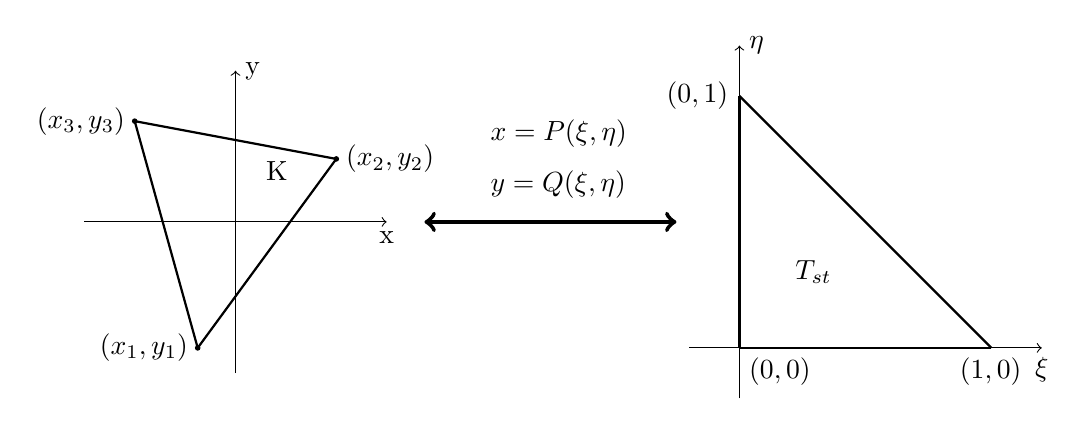
\begin{tikzpicture}[scale=1.6]
	\begin{scope}
	\draw[thin,->] (-1.2,0) -- (1.2,0) node[anchor=north] {x};
	\draw[thin,->] (0,-1.2) -- (0,1.2) node[anchor=west] {y};
	
	\draw[thick] (-0.3,-1) -- (0.8,0.5);
	\draw[thick] (0.8,0.5) -- (-0.8,0.8);
	\draw[thick] (-0.8,0.8) -- (-0.3,-1);
	
	\filldraw[black] (-0.3,-1) circle (0.5pt) node[anchor=east] {$(x_1,y_1)$};
	\filldraw[black] (0.8,0.5) circle (0.5pt) node[anchor=west] {$(x_2,y_2)$};
	\filldraw[black] (-0.8,0.8) circle (0.5pt) node[anchor=east] {$(x_3,y_3)$};
	
	\node[text width=0.5cm] at (0.4,0.4) {K};
	\end{scope}
	
	\begin{scope}[xshift=2.5cm]
	\node[anchor=east] at (-1,0) (A) {};
	\node[anchor=west] at (1,0) (B) {};
	\draw (B) edge[ultra thick,<->] (A);
	\node[text width=2cm] at (0.15,0.3) {$y=Q(\xi,\eta)$};
	\node[text width=2cm] at (0.15,0.7) {$x=P(\xi,\eta)$};
	\end{scope}
	
	\begin{scope}[xshift=4cm,yshift=-1cm,scale=2]
	\draw[thin,->] (-0.2,0) -- (1.2,0) node[anchor=north] {$\xi$};
	\draw[thin,->] (0,-0.2) -- (0,1.2) node[anchor=west] {$\eta$};
	
	\draw[thick] (0,0) -- (0,1);
	\draw[thick] (0,0) -- (1,0);
	\draw[thick] (1,0) -- (0,1);
	
	%	\filldraw[black] (0,0) circle (0.5pt) node[anchor=north west] {$(0,0)$};
	%	\filldraw[black] (0,1) circle (0.5pt) node[anchor=east] {$(0,1)$};
	%	\filldraw[black] (1,0) circle (0.5pt) node[anchor=north] {$(1,0)$};
	
	\node[anchor=north west,text width=0.8cm] at (0,0) {$(0,0)$};
	\node[anchor=east,text width=0.8cm] at (0,1) {$(0,1)$};
	\node[anchor=north,text width=0.8cm] at (1,0) {$(1,0)$};
	
	\node[text width=0.5cm] at (0.3,0.3) {$T_{st}$};
	\end{scope}
	\end{tikzpicture}
\caption{Linear mapping between $K$ and $T_{st}$.}
\end{figure}
Such a mapping can be achieved conveniently by using the nodal shape functions given by \eqref{5.210}-\eqref{5.212} as follows.

Consider the following linear mapping $\widehat S$.
\begin{align}
\widehat S:{\mathbb{R}^2} &\to {\mathbb{R}^2}\\
\left( {\xi ,\eta } \right) &\mapsto \left( {x,y} \right): = \widehat S\left( {\xi ,\eta } \right) = \left( {{{\widehat S}_1}\left( {\xi ,\eta } \right),{{\widehat S}_2}\left( {\xi ,\eta } \right)} \right)
\end{align}
where $\widehat{S}_1,\widehat{S}_2$ are defined by
\begin{align}
{\widehat S_1}\left( {\xi ,\eta } \right) =&\ \sum\limits_{i = 1}^3 {{x_i}{N_i}\left( {\xi ,\eta } \right)} \\
 =&\ {x_1} + \left( {{x_2} - {x_1}} \right)\xi  + \left( {{x_3} - {x_1}} \right)\eta \\
{\widehat S_2}\left( {\xi ,\eta } \right) =&\ \sum\limits_{i = 1}^3 {{y_i}{N_i}\left( {\xi ,\eta } \right)} \\
=&\ {y_1} + \left( {{y_2} - {y_1}} \right)\xi  + \left( {{y_3} - {y_1}} \right)\eta 
\end{align}
It is easy to verify that $\widehat{S}$ transforms the standard triangle $T_{st}$ into the triangular element $K$, i.e.,
\begin{align}
\widehat S:{T_{st}} \mapsto K
\end{align}
Then we have
\begin{align}
\label{5.220}
\iint_K {f\left( {x,y} \right)dxdy} = \iint_{{T_{st}}} {f\left( {{{\widehat S}_1}\left( {\xi ,\eta } \right),{{\widehat S}_2}\left( {\xi ,\eta } \right)} \right)\left| {\widehat J\left( {\xi ,\eta } \right)} \right|d\xi d\eta }
\end{align}
where ${\widehat J\left( {\xi ,\eta } \right)}$ is the Jacobian of the transformation, namely,
\begin{align}
\widehat J\left( {\xi ,\eta } \right) =&\ \frac{{\partial \left( {x,y} \right)}}{{\partial \left( {\xi ,\eta } \right)}}\\
=&\ \det \left[ {\begin{array}{*{20}{c}}
{\dfrac{{\partial x}}{{\partial \xi }}}&{\dfrac{{\partial x}}{{\partial \eta }}}\\
{\dfrac{{\partial y}}{{\partial \xi }}}&{\dfrac{{\partial y}}{{\partial \eta }}}
\end{array}} \right]
\end{align}
Thus,
\begin{align}
\left| {\widehat J\left( {\xi ,\eta } \right)} \right| =&\ \left| {\frac{{\partial {{\widehat S}_1}}}{{\partial \xi }}\left( {\xi ,\eta } \right) \cdot \frac{{\partial {{\widehat S}_2}}}{{\partial \eta }}\left( {\xi ,\eta } \right) - \frac{{\partial {{\widehat S}_1}}}{{\partial \eta }}\left( {\xi ,\eta } \right) \cdot \frac{{\partial {{\widehat S}_2}}}{{\partial \xi }}\left( {\xi ,\eta } \right)} \right|\\
 =&\ \left| {\left( {{x_2} - {x_1}} \right) \cdot \left( {{y_3} - {y_1}} \right) - \left( {{x_3} - {x_1}} \right) \cdot \left( {{y_2} - {y_1}} \right)} \right|\\
 =&\ \left| {{x_1}\left( {{y_2} - {y_3}} \right) + {x_2}\left( {{y_3} - {y_1}} \right) + {x_3}\left( {{y_1} - {y_2}} \right)} \right|\\
 =&\ 2\left| K \right|,\mbox{ Shoelace formula}
\end{align}
where $\left| K \right|$ denotes the area of $K$.\index{Shoelace formula}

Hence, \eqref{5.220} becomes
\begin{align}
\iint_K {f\left( {x,y} \right)dxdy} = 2\left| K \right|\iint_{{T_{st}}} {f\left( {{{\widehat S}_1}\left( {\xi ,\eta } \right),{{\widehat S}_2}\left( {\xi ,\eta } \right)} \right)d\xi d\eta }
\end{align}
Applying the Gaussian quadrature of degree $N$ for the standard triangular element $T_{st}$ yields the following result.\\
\\
\textsc{Gaussian Quadrature of Degree $N$ for General Triangular Elements $K$.}
\begin{align}
\iint_K {f\left( {x,y} \right)dxdy} \approx \left| K \right|\sum\limits_{i = 1}^{{N_T}} {{w_{{N_T},i}}f\left( {{{\widehat S}_1}\left( {{\xi _{{N_T},i}},{\eta _{{N_T},i}}} \right),{{\widehat S}_2}\left( {{\xi _{{N_T},i}},{\eta _{{N_T},i}}} \right)} \right)} 
\end{align}
\textbf{Remark 5.11.} Note that the inverse ${\widehat S^{ - 1}}$ of the transformation $\widehat{S}$ is not needed, but it can be found that
\begin{align}
{\widehat S^{ - 1}}:K &\to {T_{st}}\\
\left( {x,y} \right) &\mapsto \left( {\xi ,\eta } \right): = {\widehat S^{ - 1}}\left( {x,y} \right) = \left( {\widehat S_1^{ - 1}\left( {x,y} \right),\widehat S_2^{ - 1}\left( {x,y} \right)} \right)
\end{align}
where 
\begin{align}
\widehat S_1^{ - 1}\left( {x,y} \right) =&\ \frac{{\left( {{y_3} - {y_1}} \right)\left( {x - {x_1}} \right) - \left( {{x_3} - {x_1}} \right)\left( {y - {y_1}} \right)}}{{2\left| K \right|}}\\
\widehat S_2^{ - 1}\left( {x,y} \right) =&\ \frac{{\left( {{y_1} - {y_2}} \right)\left( {x - {x_1}} \right) + \left( {{x_2} - {x_1}} \right)\left( {y - {y_1}} \right)}}{{2\left| K \right|}}
\end{align}
\section{Multi-Dimensional Gaussian Quadrature in Standard Quadrilateral $R_{st}$}
Proceeding as two-dimensional case, we apply \eqref{4.1} to a $d$-dimensional integral on a canonical ${\left[ { - 1,1} \right]^n}$ box element yields the approximation
\begin{align}
&\int_{ - 1}^1 { \cdots \int_{ - 1}^1 {f\left( {{x_1}, \ldots ,{x_d}} \right)d{x_1} \cdots d{x_d}} } \\
& \approx \int_{ - 1}^1 { \cdots \int_{ - 1}^1 {\left( {\sum\limits_{{i_1} = 1}^{{n_1}} {{w_{{n_1},{i_1}}}f\left( {{x_{{n_1},{i_1}}},{x_2}, \ldots ,{x_d}} \right)} } \right)d{x_2} \cdots d{x_d}} } \\
=&\ \sum\limits_{{i_1} = 1}^{{n_1}} {{w_{{n_1},{i_1}}}\int_{ - 1}^1 { \cdots \int_{ - 1}^1 {f\left( {{x_{{n_1},{i_1}}},{x_2}, \ldots ,{x_d}} \right)d{x_2} \cdots d{x_d}} } } \\
& \approx \sum\limits_{{i_1} = 1}^{{n_1}} {{w_{{n_1},{i_1}}}\int_{ - 1}^1 { \cdots \int_{ - 1}^1 {\left( {\sum\limits_{{i_2} = 1}^{{n_2}} {{w_{{n_2},{i_2}}}f\left( {{x_{{n_1},{i_1}}},{x_{{n_2},{i_2}}},{x_3}, \ldots ,{x_d}} \right)} } \right)d{x_3} \cdots d{x_d}} } } \\
=&\ \sum\limits_{{i_1} = 1}^{{n_1}} {\sum\limits_{{i_2} = 1}^{{n_2}} {{w_{{n_1},{i_1}}}{w_{{n_2},{i_2}}}\int_{ - 1}^1 { \cdots \int_{ - 1}^1 {f\left( {{x_{{n_1},{i_1}}},{x_{{n_2},{i_2}}},{x_3}, \ldots ,{x_d}} \right)d{x_3} \cdots d{x_d}} } } } \\
& \approx  \cdots \\
& \approx \sum\limits_{{i_1} = 1}^{{n_1}} {\sum\limits_{{i_2} = 1}^{{n_2}}  \cdots  \sum\limits_{{i_d} = 1}^{{n_d}} {\prod\limits_{j = 1}^d {{w_{{n_j},{i_j}}}} f\left( {{x_{{n_1},{i_1}}}, \ldots ,{x_{{n_d},{i_d}}}} \right)} } 
\end{align}
for some positive integers $n_1,\ldots,n_d$.

Define
\begin{align}
{E_{{n_1}, \ldots ,{n_d}}}\left\{ f \right\}: =&\ \int_{ - 1}^1 { \cdots \int_{ - 1}^1 {f\left( {{x_1}, \ldots ,{x_d}} \right)d{x_1} \cdots d{x_d}} }  \\
&- \sum\limits_{{i_1} = 1}^{{n_1}} {\sum\limits_{{i_2} = 1}^{{n_2}}  \cdots  \sum\limits_{{i_d} = 1}^{{n_d}} {\prod\limits_{j = 1}^d {{w_{{n_j},{i_j}}}} f\left( {{x_{{n_1},{i_1}}}, \ldots ,{x_{{n_d},{i_d}}}} \right)} } 
\end{align}
\textbf{Problem 6.1.} \textit{Given $f \in {C^n}\left( {{{\left[ { - 1,1} \right]}^d}} \right)$, where $n = \max \left\{ {{n_i}:i = 1, \ldots ,d} \right\}$. Prove that }
\begin{align}
{E_{{n_1}, \ldots ,{n_d}}}\left\{ f \right\} \le {2^{d - 1}}\sum\limits_{i = 1}^d {\frac{2}{{\left( {2{n_i} + 1} \right)!}}{{\left( {\frac{{{2^{{n_i}}}{{\left( {{n_i}!} \right)}^2}}}{{\left( {2{n_i}} \right)!}}} \right)}^2}{{\left\| {\frac{{{\partial ^{2{n_i}}}f}}{{\partial x_i^{{2n_i}}}}} \right\|}_{{L^\infty }\left( {\left[ { - 1,1} \right]} \right)}}} 
\end{align}
\textsc{Hint.} The main idea is to use induction and the following identity
\begin{align}
\sum\limits_{i = 1}^n {{w_{n,i}}}  = 2,\hspace{0.2cm}\forall n \in {\mathbb{Z}^ + }
\end{align}
See Sec. 4.1. \hfill $\square$\\
\\
\textbf{Corollary 6.2.} \textit{Given $f \in {C^n}\left( {{{\left[ { - 1,1} \right]}^d}} \right)$, then}
\begin{align}
{E_{\underbrace {n, \ldots ,n}_{d's}}}\left\{ f \right\} \le \frac{{{2^d}d}}{{\left( {2n + 1} \right)!}}{\left( {\frac{{{2^n}{{\left( {n!} \right)}^2}}}{{\left( {2n} \right)!}}} \right)^2}{\left\| {\frac{{{\partial ^{2n}}f}}{{\partial x_i^{2n}}}} \right\|_{{L^\infty }\left( {\left[ { - 1,1} \right]} \right)}}
\end{align}

\section{\textsc{Matlab} Implementation}
\subsection{Legendre Polynomials}
The command, see \cite{3},
\begin{verbatim}
legendreP(n,x)
\end{verbatim}
returns the $n$th degree Legendre polynomial\index{Legendre polynomial} at $x$.

To plot Legendre polynomials of order 1 through 5, we use the following \textsc{Matlab} script
\begin{verbatim}
syms x y
fplot(legendreP(1:6, x))
axis([-1.5 1.5 -1 1])
grid on

ylabel('P_n(x)')
title('Legendre polynomials of degrees 1 through 6')
legend('1','2','3','4','5','6','Location','best')
\end{verbatim}
to obtain
\begin{figure}[H]
\centering
\includegraphics[scale=0.85]{2}
\caption{Legendre polynomials of degree 1 through 6.}
\end{figure}

Use \texttt{vpasolve} to find the roots of the Legendre polynomial of degree 7.
\begin{verbatim}
syms x
roots = vpasolve(legendreP(7,x) == 0)
\end{verbatim}
\subsection{Gaussian Quadrature}
\subsubsection{One-Dimensional Gaussian Quadrature}
\footnote{Source: \url{https://www.mathworks.com/}.}
\begin{verbatim}
function [I]=LGQ(f,N,a,b)
N=N-1;
N1=N+1;
N2=N+2;
xu=linspace(-1,1,N1)';
% Initial guess
y=cos((2*(0:N)'+1)*pi/(2*N+2))+(0.27/N1)*sin(pi*xu*N/N2);
% Legendre-Gauss Vandermonde Matrix
L=zeros(N1,N2);
% Derivative of LGVM
Lp=zeros(N1,N2);
% Compute the zeros of the N+1 Legendre Polynomial
% using the recursion relation and the Newton-Raphson method
y0=2;
% Iterate until new points are uniformly within epsilon of old points
while max(abs(y-y0))>eps
    L(:,1)=1;
    Lp(:,1)=0;
    L(:,2)=y;
    Lp(:,2)=1;
    for k=2:N1
        L(:,k+1)=( (2*k-1)*y.*L(:,k)-(k-1)*L(:,k-1) )/k;
    end
    Lp=(N2)*( L(:,N1)-y.*L(:,N2) )./(1-y.^2);
    y0=y;
    y=y0-L(:,N2)./Lp;
end
% Linear map from[-1,1] to [a,b]
v=(a*(1-y)+b*(1+y))/2;
% Compute the weights
w=(b-a)./((1-y.^2).*Lp.^2)*(N2/N1)^2;
% Compute the approximation
I=sum(double(subs(f,v)).*w);
\end{verbatim}
\subsubsection{Two-Dimensional Gaussian Quadrature}
\footnote{Source: \url{https://www.mathworks.com/}}
\begin{verbatim}
function [X,Y,Wx,Wy]=triquad(N,v)
n=1:N;
nnk=2*n+1;
A=[1/3 repmat(1,1,N)./(nnk.*(nnk+2))];
n=2:N;
nnk=nnk(n);
B1=2/9;
nk=n+1;
nnk2=nnk.*nnk;
B=4*(n.*nk).^2./(nnk2.*nnk2-nnk2);
ab=[A' [2; B1; B']]; s=sqrt(ab(2:N,2));
[V,X]=eig(diag(ab(1:N,1),0)+diag(s,-1)+diag(s,1));
[X,I]=sort(diag(X));
x=(X+1)/2;
wx=ab(1,2)*V(1,I)'.^2/4;

N=N-1;
N1=N+1;
N2=N+2;
y=cos((2*(N:-1:0)'+1)*pi/(2*N+2));
L=zeros(N1,N2);
y0=2;
iter=0;
while max(abs(y-y0))>eps
    L(:,1)=1;
    L(:,2)=y;
    for k=2:N1
        L(:,k+1)=( (2*k-1)*y.*L(:,k)-(k-1)*L(:,k-1) )/k;
    end
    Lp=(N2)*(L(:,N1)-y.*L(:,N2))./(1-y.^2);
    y0=y;
    y=y0-L(:,N2)./Lp;
    iter=iter+1;
end

cd=[ 1, 0, 0; -1, 0, 1; 0, 1,-1]*v;
t=(1+y)/2;
Wx=abs(det(cd(2:3,:)))*wx;
Wy=1./((1-y.^2).*Lp.^2)*(N2/N1)^2;
[tt,xx]=meshgrid(t,x); yy=tt.*xx;
X=cd(1,1)+cd(2,1)*xx+cd(3,1)*yy;
Y=cd(1,2)+cd(2,2)*xx+cd(3,2)*yy;
\end{verbatim}
Try them!\\
\\
\\
\\
\begin{center}
\textsc{The End}
\end{center}
\newpage
\printindex
\newpage
\begin{thebibliography}{999}
\bibitem {1} Richard L. Burden, J. Douglas Faires, \textit{Numerical Analysis}, Ninth Edition.
\bibitem {pde} G. Evans, J. Blackledge, P. Yardley, \textit{Analytic Methods for Partial Differential Equations}, Springer.
\bibitem {6} Eugene Isaacson, Herbert Bishop Keller, \textit{Analysis of Numerical Methods}, Dover Publications, Inc., New York.
\bibitem {7} Math 5172 - Finite Element Method, \textit{Quadrature Formulas in Two Dimensions}, Section 001, Spring 2010.
\bibitem {2} \url{https://www.nguyenquanbahong.com/2017/01/21/problem-system-equations-relating-gaussian-quadrature-formulas/}
\bibitem {3} \url{https://www.mathworks.com/help/symbolic/legendrep.html}
\bibitem {4} \url{https://en.wikipedia.org/wiki/Legendre_polynomials}
\bibitem {5} \url{https://en.wikipedia.org/wiki/Gaussian_quadrature}
\end{thebibliography}
\end{document}